%% LyX 1.5.1 created this file.  For more info, see http://www.lyx.org/.
%% Do not edit unless you really know what you are doing.
\documentclass[english]{book}
\usepackage[T1]{fontenc}
\usepackage[latin9]{inputenc}
\pagestyle{headings}
\setcounter{secnumdepth}{3}
\setcounter{tocdepth}{3}
\usepackage{float}
\usepackage{textcomp}
\usepackage{graphicx}
\usepackage{epsf}
\usepackage{caption}
\usepackage{amssymb}
\usepackage{amsmath}
\usepackage{natbib}
\usepackage{color}
\usepackage{array}
\bibliographystyle{plainnat}

\IfFileExists{url.sty}{\usepackage{url}}
                      {\newcommand{\url}{\texttt}}

\makeatletter

%%%%%%%%%%%%%%%%%%%%%%%%%%%%%% LyX specific LaTeX commands.
%% Bold symbol macro for standard LaTeX users
\providecommand{\boldsymbol}[1]{\mbox{\boldmath $#1$}}

%% Because html converters don't know tabularnewline
\providecommand{\tabularnewline}{\\}

%%%%%%%%%%%%%%%%%%%%%%%%%%%%%% Textclass specific LaTeX commands.
\newenvironment{lyxcode}
{\begin{list}{}{
\setlength{\rightmargin}{\leftmargin}
\setlength{\listparindent}{0pt}% needed for AMS classes
\raggedright
\setlength{\itemsep}{0pt}
\setlength{\parsep}{0pt}
\normalfont\ttfamily}%
 \item[]}
{\end{list}}

%%%%%%%%%%%%%%%%%%%%%%%%%%%%%% User specified LaTeX commands.
%% LyX 1.5.1 created this file.  For more info, see http://www.lyx.org/.
%% Do not edit unless you really know what you are doing.
\usepackage{float}
\usepackage{textcomp}
\usepackage{color}
\IfFileExists{url.sty}{\usepackage{url}
}
                      {\newcommand{\url}{\texttt}}
\makeatletter

%%%%%%%%%%%%%%%%%%%%%%%%%%%%%% LyX specific LaTeX commands.
%% Bold symbol macro for standard LaTeX users


%% Because html converters don't know tabularnewline


%%%%%%%%%%%%%%%%%%%%%%%%%%%%%% Textclass specific LaTeX commands.


%%%%%%%%%%%%%%%%%%%%%%%%%%%%%% User specified LaTeX commands.
%% LyX 1.5.4 created this file.  For more info, see http://www.lyx.org/.
%% Do not edit unless you really know what you are doing.

\usepackage{float}
\usepackage{textcomp}
\usepackage{url}
\makeatletter

%%%%%%%%%%%%%%%%%%%%%%%%%%%%%% LyX specific LaTeX commands.
%% Bold symbol macro for standard LaTeX users


%% Because html converters don't know tabularnewline


%%%%%%%%%%%%%%%%%%%%%%%%%%%%%% Textclass specific LaTeX commands.


%%%%%%%%%%%%%%%%%%%%%%%%%%%%%% User specified LaTeX commands.
%% LyX 1.5.4 created this file.  For more info, see http://www.lyx.org/.
%% Do not edit unless you really know what you are doing.



\usepackage{geometry}
\geometry{verbose,letterpaper,tmargin=1in,bmargin=1in,lmargin=1in,rmargin=1in}
\usepackage{float}
\usepackage{textcomp}
\usepackage{url}

\makeatletter

%%%%%%%%%%%%%%%%%%%%%%%%%%%%%% LyX specific LaTeX commands.
%% Bold symbol macro for standard LaTeX users



%%%%%%%%%%%%%%%%%%%%%%%%%%%%%% Textclass specific LaTeX commands.


%%%%%%%%%%%%%%%%%%%%%%%%%%%%%% User specified LaTeX commands.
\usepackage{hyperref}

\let\myUrl\url
\renewcommand{\url}[1]{(\myUrl{#1})}

\makeatother
\makeatother
\makeatother

\usepackage{babel}
\makeatother

\begin{document}
\noindent \begin{center}
\thispagestyle{empty}%
\begin{figure}[H]
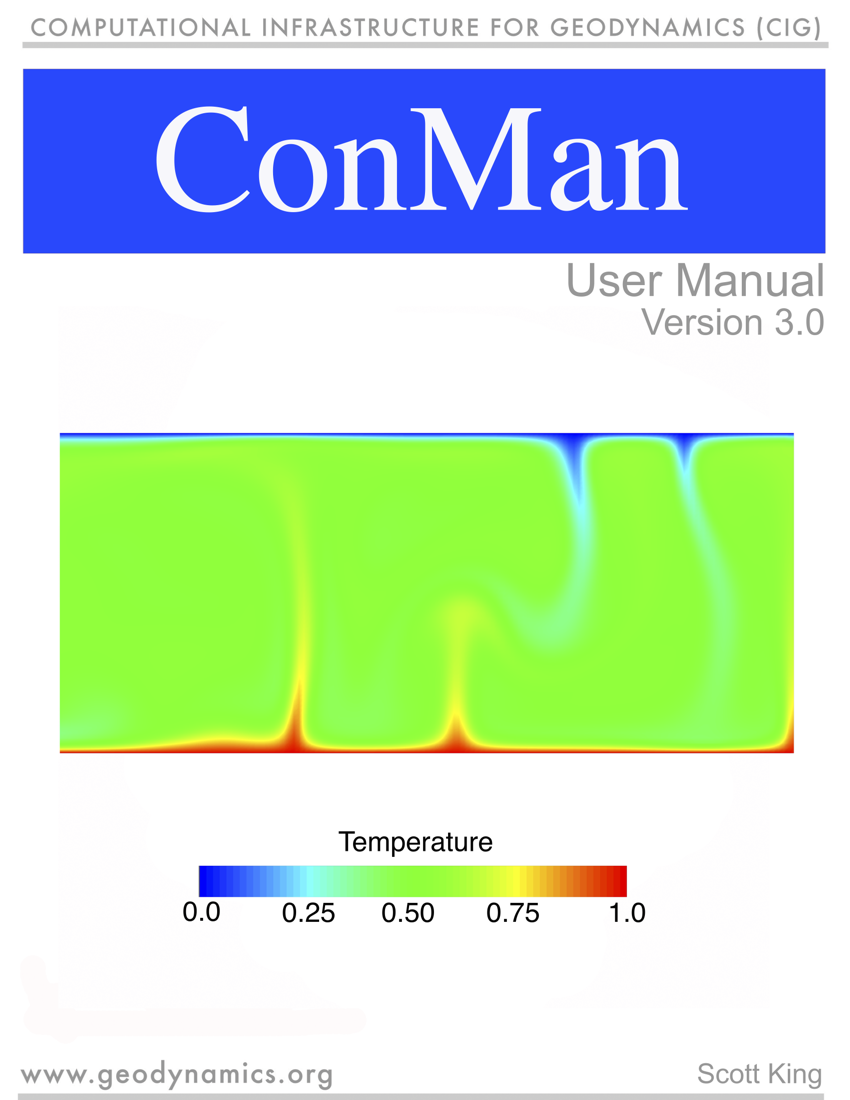
\includegraphics[width=0.75\paperwidth]{images/conman_cover.png} 
\end{figure}

\par\end{center}


\title{ConMan}

\author{
Version 3.0 \\
\\
\\
 Scott King\\
\\
\date{\today}
\\
\copyright  2019 Computational Infrastructure for Geodynamics
 }
 
\maketitle
\tableofcontents{}

\listoffigures

\raggedbottom

\newpage{}

\chapter{Preface}

\section{Abstract}

This manual serves as a user guide for ConMan, a finite element program for the solution of the equations of compressible and incompressible, infinite-Prandtl number convection in two dimensions originally written by Arthur Raefsky, Scott King, and Brad Hager \citep{king90a}. 
Changyeol Lee contributed significantly to the compressible formulation in this distribution \citep{lee09}.
The 3.0 version of ConMan solves the Bousinessq (BA), Extended Bousinessq (EBA), Trucated Anelastic Liquid (TALA), and Anelastic Liquid (ALA) approximations \citep{king10}.  

ConMan has always been a public domain program and is maintained and distributed by the Computational Infrastructure for Geodynamics (CIG) geodynamics.org and is made available under the GNU General Pubic License either version 2 or later.

ConMan is written in FORTRAN making use of FORTRAN's memory allocation and has been tested on a variety of linux systems with gfortran and intel fortan compilers. 
It has been benchmarked against other existing codes (see Chapter \ref{cha:The-Benchmark-Cases}).
Yet as with anything free, it comes with no guarantees. 
The authors would appreciate any information regarding bugs or potential problems but make no promises regarding the timeliness of changes or fixes; see Section \ref{sec:Support} for instructions on how to report problems.

\section{Changes Since Version 2.0}

There are several significant differences that the user familiar with past versions of ConMan will find in the 3.0 version.  
First, we removed the clunky memory manager library (a set of routines wrapped around the c function malloc) and replaced them with FORTRAN 90's allocate and deallocate functions.
This eliminates many of the compilation problems people experienced with the 2.0 version. 
Most of these routines were in files subroutines input and elminp. 

As part of a general clean up, we replaced the separate input and elminp (both input subroutines) and created a new input subroutine.
As part of this we removed the `element library' function (eglib.F and eg2.F) which was a structure originally designed for different formulations 2D Cartesian, 3D Cartesian, spherical axysymmetric, ...).
Because these were never fully developed, it made on sense to retain the cumbersome structure.
We also moved all out the subroutines associated with output, into new output subroutine.
The user does not need to hunt through the time\_driver subroutine to find out where the specific output subroutines are called.
Thus, subroutines geoid, fluxke, masflx, print, output\_rheol, print\_compbm\_data, and stress are all in subroutine output.

We also changed the names of many of the subroutines to take advantage of longer subroutine names allowed by modern FORTRAN.  
Thus f\_tlhs has become form\_temp\_matrix, f\_vres has become form\_vel-ocity\_rhs, f\_vstf has become form\_velocity\_stiffness\_matrix.  
Similarly, subroutine timdrv has become time\_driver. 
As you look through the code there are examples where this could have been carried further.

Second, Picard iteration for the temperature equation is now a runtime option as opposed to a compiler option.
This necessitated specifying both implicit and explicit subroutines for the temperature right hand side, form\_temp\_rhs\_implicit and form\_temp\_rhs\_explicit
As well as a form\_temp\_matrix.F for the implicit temperature matrix and form\_temp\_mass\_matrix for the lumped mass matrix that has traditionally been used for the explicit version of the temperature solver.

Third, we added the EBA, TALA, and ALA formulations as described in \citet{king10}.  
The compressible formulation is described in Chapter \ref{chap:compress}. 
This required a number of changes throughout the form\_temperature and form\_velocity subroutines.
We provide a test suite that runs a subset of the problems from \citet{king10} that can be used to verify the installation version 3.0.  

Finally, we have added a cookbook of subduction wedge problems based on problems from the subduction zone benchmark paper \citep{vanKeken08} and one based on the compressible convection benchmark paper \citep{king10}.
This required adding a new 'fault' subroutine and a subroutine to implement the Batchelor corner flow boundary conditions.
These can be found in the subduct.src directory.

\section{Introduction}

This manual contains all of the necessary information for setting up input and running ConMan. 
It assumes some familiarity with the finite element method and FORTRAN. An excellent reference book for more detail on the finite element method is \citet{hughes87}. 
All of the data structures and bookkeeping arrays in ConMan follow the conventions in Hughes so for the person who wishes to make extensive use of ConMan, this book is a worthwhile investment.

This manual is broken up into several parts: it begins with a brief introduction to the finite element method and the notation that is used throughout the manual and ConMan. 
There is a discussion of the equations solved and the material properties including how and where to modify the code. 
There is also discussion of some key points concerning the implementation and finally a description of all the input variables. 
Within this document the following convention will be followed: subroutine names from ConMan will be given in \textbf{bold} type, variables from ConMan will be given in \emph{italicized} type.

\section{Contributors}

ConMan was originally developed by Scott King, Arthur Raefsky, and Brad Hager \citep{king90b}. 
The grid generation routines were adapted from DLEARN, a code distributed with \citet{hughes87}.
Numerous people have contributed to ConMan and related codes over the past 25 years, including: Louise H. Kellogg and Walter Kiefer (SCAM - Spherical Convection in an Axisymmetric Mantle), Cinzia G. Farnetani (cylindical version for plumes), Junan Chen, Steve S. Shapiro (marker chain and field methods), Mark Simons (geoid calculation), Peter Puster (cylindical version), Don E. Koglin (rheology and plates), Hannah L. Redmond (SCAM - Spherical Convection in an Axisymmetric Mantle), Peter van Keken (Picard iteration and benchmarking), Changyeol Lee and Ikuko Wada (compressible formulations and subduction problems).
This distribution only includes the Cartesian version and does not include markers, marker chains or compositional fields.
These could easily be added and I have the older routines if someone it interested in merging those features with the current code.

\section{Citation}

The ConMan team requests that in your oral presentations and in your papers that you indicate your use of this code by citing these two papers which describe the methods the code is based on:

\begin{itemize}
\item King, S.D., A. Raefsky, and B.H. Hager (1990), ConMan: Vectorizing
a finite element code for incompressible two-dimensional convection
in the Earth's mantle, \emph{Phys. Earth Planet. Int., 59,} 195-208. 
\end{itemize}

\begin{itemize}
\item King S. D., C. Lee, P. E. van Keken, W. Leng, S. Zhong, E. Tan, E., M. Gurnis, N. Tosi, and M. C. Kameyama (2010) A community benchmark for 2D Cartesian compressible convection in the Earth's mantle, \emph{Geophys. J. Int., 180,} 73-87, 2010. doi:10.1111/j.1365-246X.2009.04413.x 
\end{itemize}

\begin{itemize}
\item King, S. D., A. Raefsky, and B.H. Hager (2020), ConMan v3.0.0 [software], doi:10.5281/zenodo.3633152.
\end{itemize}

\section{Support}

ConMan is freely available from the Computational Infrastructure for Geodynamics (CIG) \url{geodynamics.org} under the GPL 2.0 or later license (Appendix A)
%is making this source code available to you 
in the hope that the software will enhance your research in geophysics. 
Maintenance is supported by a grant from the National Science Foundation to CIG, managed by the University of California at Davis. 

Please acknowledge CIG as follows:
\begin{itemize}
\item ConMan is hosted by the Computational Infrastructure for Geodynamics (CIG) which is supported by the National Science Foundation under awards EAR-0949446 and EAR-1550901.
\end{itemize}

ConMan code was donated to CIG in June 2008.  
\\

Any opinions, findings, and conclusions or recommendations expressed
in this material are those of the author and do not necessarily reflect
the views of the National Science Foundation.


\chapter{Computational Approach}

\section{The Finite Element Method}

This section closely follows \citet[][Chapter~1, sections 1-4]{hughes87}. There are two ways we can write the equation,
the strong and the weak form. More readers are probably more familiar
with the strong form, and less familiar with the weak form. The finite
element method is cast in the weak form. In elasticity, for example,
the weak form comes from a variational principal, such as the principal
of virtual displacements in elasticity. For viscous flow, there is
also a variational form, but we will not discuss that here.

In general, the finite element method takes a differential equation
(strong form) and transforms it into an integral equation (weak form).


\subsection{The Strong Form}

For example, the strong form of this simple equation is stated as
follows:

Given $f\left(x\right):\left[0,1\right]$ $\rightarrow\Re$ and constants
\emph{g} and \emph{h}, find $u:\left[0,1\right]\rightarrow\Re$, such
that

\begin{equation}
u,_{xx}\left(x\right)+f\left(x\right)=0
\end{equation}

\begin{equation}
u\left(1\right)=g\label{eq:}
\end{equation}

\begin{equation}
-u,_{x}\left(0\right)=h
\end{equation}

\noindent This choice of initial conditions allows us to examine both
kinds of boundary conditions. The solution is trivial, but that does
not matter. For completeness, it is 
\begin{equation}
u(x)=g+(1-x)h+\int_{x}^{1}\left(\int_{0}^{y}f(z)dz\right)dy
\end{equation}

\subsection{The Weak Form}

The weak form of the corresponding boundary value problem is stated:

Given \emph{f}, \emph{g} and \emph{h}, as before. Find $u\left(x\right)\epsilon\mathcal{L}$
such that for all $w\left(x\right)\epsilon\nu$

\begin{equation}
\intop_{0}^{1}w,_{x}\left(x\right)u,_{x}\left(x\right)=\intop_{0}^{1}w\left(x\right)f\left(x\right)dx+w\left(0\right)h\end{equation}


\noindent $\nu$ is the set of weighting functions defined by

\begin{equation}
\nu=\left\{ w\left(x\right)|w\left(x\right)\epsilon H^{1},\, w\left(1\right)=0\right\} \end{equation}


\noindent and $\mathcal{L}$ is a set of trial solutions defined by

\begin{equation}
\mathcal{L=\left\{ \mathrm{\mathit{u\left(x\right)|u\left(x\right)}\epsilon H^{1},\,\mathit{u}\left(1\right)=\mathit{g}}\right\} }
\end{equation}


\noindent $H^{1}$ is the set of all functions whose first derivatives
are square integrable on {[}0, 1]. The integral equation is then solved
by integrating over each element in the domain and adding the result.
The result is a large sparse matrix equation of the form

\begin{equation}
\left[K\right]x=b
\end{equation}

\noindent where \emph{{[}K]} is referred to as the element stiffness
matrix. There will be more to say about the implementation in Section
\ref{cha:Input-Guide}.

\subsection{Galerkin's Approximation}

Now we have a start on the finite element method. We continue to follow
Hughes; however, his notation becomes quite difficult to keep up with.
Now, let's begin to think about putting a solution on the computer.
Because we will have a finite approximation, related to how fine we
space our grid, our solution will only approximate the real solution.
Following Hughes' notation, the solution on the grid will be denoted
as $u^{h}$ where $h$ is some measure of the spacing at the grid.
Then, \begin{equation}
\int_{0}^{1}w^{h},_{x}u^{h},_{x}dx~=~\int_{0}^{1}w^{h}\, f^{h}\, dx+w^{h}(0)h.\label{eq:weak}
\end{equation}
 approximates our exact solution $u$.

On a computer, we don't have a continuous solution. We have a solution
at discrete points. We need to approximate the solution between the
points (in order to integrate over the function). We will do this
with \textbf{shape functions}, as they are usually called in the finite
element language. Hughes uses $N_{A}A=1,2,\cdots,n$ to denote the
shape functions. You can also think of these as basis functions or
interpolation functions. We require $N_{A}(1)=0,A=1,2,\cdots,n$.
In order to specify our boundary condition, we need another shape
function which has the property 
\begin{equation}
N_{n+1}(1)=1.
\end{equation}
Then, $g^{h}$ is given by, 
\begin{equation}
g^{h}=gN_{n+1}
\end{equation}
and thus, 
\begin{equation}
g^{h}(1)=g.
\end{equation}
With these definitions, we can write our solution $u^{h}$ as 
\begin{equation}
u^{h}=\sum_{A=1}^{n}\, d_{A}\, N_{A}+gN_{n+1}
\end{equation}
where the $d_{A}$'s are unknown constants to be solved for.

In the next section we will make the shape functions more concrete.
It is useful to see how general this is, because in principle there
is a great deal of flexibility in how we choose the shape functions.

We have not said anything more about this function $w^{h}$ and how
we are going to choose it. If our shape functions form a basis set
for the grid, then we can represent \textbf{any} function as a sum
of the basis functions times some arbitrary coefficients $c_{i}$,
\begin{equation}
w^{h}=\sum_{A=1}^{n}\, c_{A}\, N_{A}=c_{1}\, N_{1}~+~c_{2}\, N_{2}~+~\cdots~+~c_{n}\, N_{n}\label{eq:whapprox}
\end{equation}
 If you don't remember this part of your mathematics background think
about Fourier series. Any one-dimensional function can be represented
as an infinite series of sines and cosines times some unique set of
coefficients. The shape functions form a similar kind of basis set.

Notice that because we required that $N_{A}(1)=0,A=1,2,\cdots,n$,
Equation~\ref{eq:whapprox} satisfies the requirement that $w^{h}(1)=0$,
as necessary.

Using our definitions of the $w^{h}$'s and our approximation for
$u^{h}$, we can get the messy expression for Equation~\ref{eq:weak}
\[
\int_{0}^{1}\left(\frac{\partial}{\partial x}\left(\sum_{A=1}^{n}\, c_{A}\, N_{A}\right)\frac{\partial}{\partial x}\left(\sum_{B=1}^{n}\, d_{B}\, N_{B}+gN_{n+1}\right)\right)dx~=~\]
 \begin{equation}
\int_{0}^{1}\sum_{A=1}^{n}\, c_{A}\, N_{A}\, f^{h}\, dx+\sum_{A=1}^{n}\, c_{A}N_{A}(0)h.\end{equation}
 By rearranging, we can write \begin{equation}
\sum_{A=1}^{n}G_{A}c_{A}=0\end{equation}
 where \[
G_{A}~=~\int_{0}^{1}\left(\frac{\partial N_{A}}{\partial x}\right)\left(\sum_{B=1}^{n}\, d_{B}\,\frac{\partial N_{B}}{\partial x}\right)dx\]
 \begin{equation}
-\int_{0}^{1}N_{A}\, f^{h}\, dx-N_{A}(0)h+\int_{0}^{1}\frac{\partial N_{A}}{\partial x}\frac{\partial N_{n+1}}{\partial x}\, g\, dx\end{equation}
 Now I use the fact that the shape functions are basis functions,
so $N_{A}\times N_{B}$ is zero except when $A=B$. We could equally
well use the fact that the $c_{A}$'s are arbitrary. Both of these
force us to conclude that each $G_{A}$ must be identically zero and
we get \[
\sum_{B=1}^{n}\,\left(\int_{0}^{1}\frac{\partial N_{A}}{\partial x}\frac{\partial N_{B}}{\partial x}\, dx\right)\, d_{B}=\]
 \begin{equation}
\int_{0}^{1}N_{A}\, f^{h}\, dx+N_{A}(0)h-g\,\int_{0}^{1}\frac{\partial N_{A}}{\partial x}\frac{\partial N_{n+1}}{\partial x}\, dx\label{eq:feform}\end{equation}
 Everything in Equation~\ref{eq:feform} is known except the $d_{B}$'s.
This constitutes a system of $n$ equations and $n$ unknowns. We
can think of the left-hand side as a matrix, $K_{AB}$ whose entries
are \begin{equation}
\int_{0}^{1}\frac{\partial N_{A}}{\partial x}\frac{\partial N_{B}}{\partial x}\, dx\label{eq:Kelements}\end{equation}
 We can write \begin{equation}
\sum_{B=1}^{n}\, K_{AB}d_{B}=F_{A},~~~~~A=1,2,\cdots,n\end{equation}
 or as a matrix equation \begin{equation}
\left[K\right]\,\{d\}=\{f\}\end{equation}
 where \begin{equation}
[k]=\left[\begin{array}{cccc}
K_{11} & K_{12} & \cdots & K_{1n}\\
K_{21} & K_{22} & \cdots & K_{2n}\\
\vdots & \vdots &  & \vdots\\
K_{n1} & K_{n2} & \cdots & K_{nn}\end{array}\right]\label{Kmatrix}\end{equation}
 By tradition, $\left[K\right]$ is the stiffness matrix, $\{f\}$
is the force vector, and $\{d\}$ is the displacement vector. When
the problem under consideration pertains to a mechanical system, this
makes the most sense but, even in heat conduction problems, or fluid
flow problems, the terminology is still (often) retained.

\subsection{Shape Functions}

At this point, we narrow the focus to deal with specifically the elements
in ConMan. It is possible to think very general shape functions but,
in practice people use triangles or quadralaterals (in 2D). In terms
of the level of approximation, there are also a lot of possibilities.
We will stick to the simplest form, bilinear elements, but you should
be aware that higher-order elements (biquadratic or bicubic spline
elements) are also popular with some people. This section is condensing
a lot of very useful material from Chapter 3 of Hughes' book into
a short overview. If you want to see more complete derivations, proofs
of convergence, etc., of how to go about using higher-order elements,
look at Hughes book, Chapter 3.

Let's start by thinking of a rectangle that is 2a by 2b in length
centered at (0,0). There are two properties we would like the shape
functions to have \begin{eqnarray}
\sum_{A=1}^{4}N_{A}(X,Y) & = & 1\label{eq:normalize}\\
\sum_{A=1}^{4}N_{A}(X,Y)\, X_{A} & = & X\label{eq:interpx}\\
\sum_{A=1}^{4}N_{A}(X,Y)\, Y_{A} & = & Y\label{eq:interpy}\end{eqnarray}
Equation~\ref{eq:normalize} says that they are normalized, so that
they sum to one (everywhere on X,Y). Equations~\ref{eq:interpx}
and~\ref{eq:interpy} state that the shape functions are also interpolation
functions. Without doing a lot of derivation, I will claim that for
the rectangle described above, \begin{eqnarray}
N_{1} & = & \frac{(a-x)(b-y)}{4ab}\\
N_{2} & = & \frac{(a+x)(b-y)}{4ab}\\
N_{3} & = & \frac{(a+x)(b+y)}{4ab}\\
N_{4} & = & \frac{(a-x)(b+y)}{4ab}\end{eqnarray}
these shape functions satisfy the conditions in Equation~\ref{eq:normalize}
and Equations ~\ref{eq:interpx} and~\ref{eq:interpy}. A good exercise
would be to show this is true. A visual representation of these shape
functions is shown in Figure\ref{fig:bilinear}.

\begin{figure}
\begin{centering}
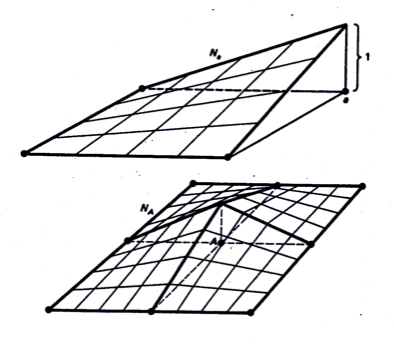
\includegraphics{images/bilinearshape.png} 
\caption{\label{fig:bilinear}The bilinear shape function for a single
element (top) and the four elements whose shape functions combine
to form the global shape function for node A (bottom). Figure taken
from Hughes, Section 3.2.}
\end{centering}
\end{figure}

In ConMan we further choose to normalize this by setting $a=0.5$ and $b=0.5$. This choice gives us an element whose area is 1, a convenient way to scale elements. 

Notice that it is easy to take the derivatives of these shape functions.  Below we write the x and y derivatives of the shape functions,
\begin{eqnarray}
N_{1,x} & = & \frac{-(0.5-y)}{1}\\
N_{2,x} & = & \frac{(0.5-y)}{1}\\
N_{3,x} & = & \frac{(0.5+y)}{1}\\
N_{4,x} & = & \frac{-(0.5+y)}{1}\end{eqnarray}
 \begin{eqnarray}
N_{1,y} & = & \frac{-(0.5-x)}{1}\\
N_{2,y} & = & \frac{-(0.5+x)}{1}\\
N_{3,y} & = & \frac{(0.5+x)}{1}\\
N_{4,y} & = & \frac{(0.5-x)}{1}\end{eqnarray}.
If we want to solve a problem on a domain that is not convenient to split into a grid of 1 by 1 unit elements, we use an important principle of mathematics, the Jacobian of the transformation
\begin{equation}
K_{11}~=~\int_{A}^{B}N_{1,x}N_{1,x}\, dx~=~\int_{0}^{1}N_{1,x}N_{1,x}\, J dx
\end{equation}
where $J$ is the Jacobian of the transformation. This is a very
powerful point. When we are thinking of solving a regular Cartesian
domain, this just corresponds to a stretching or a shrinking the shape functions above (see Figure \ref{fig:mapping}).

\begin{figure}
\begin{centering}
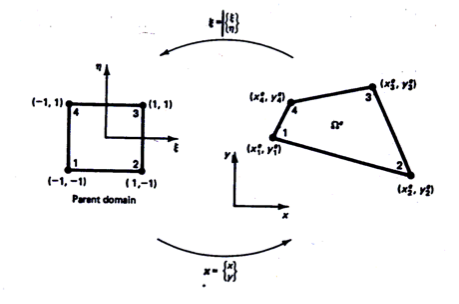
\includegraphics{images/mapping.png} 
\caption{\label{fig:mapping}The mapping between the global domain (right)
and the parent element domain (left) using the shape functions. Figure
taken from Hughes, Section 3.2.}
\end{centering}
\end{figure}

However, if we are thinking about a cylindrical geometry, for example,
we can use the Jacobian of the transformation between the geometries.
Let's look at two examples.

Converting an element 0.05 by 0.10 centered at (0.1,0.2) to the `parent
element' centered at (0,0). Hughes also uses $\xi,\eta$ for the $X,Y$
coordinate pair in the `parent element.' So we could write \begin{eqnarray}
x & = & 0.1+{0.05}\xi+0.0\eta\\
y & = & 0.2+{0.0}\xi+{0.10}\eta\end{eqnarray}
 or in matrix form we could write \begin{equation}
\left\{ \begin{array}{c}
x\\
y\end{array}\right\} =\left[\begin{array}{cc}
0.05 & 0.0\\
0.0 & 0.10\end{array}\right]\left\{ \begin{array}{c}
\xi\\
\eta\end{array}\right\} +\left\{ \begin{array}{c}
0.1\\
0.2\end{array}\right\} \label{eq:transform}\end{equation}
If the transformation was from an arbitrarily-shaped quadrilateral
to the parent element, then the off diagonal terms in the matrix in
equation~\ref{eq:transform} will not be zero. It is easy enough
to show that \begin{equation}
\int_{x_{1}}^{x_{2}}\int_{y_{1}}^{y_{2}}f(x,y)\, dx\, dy=\int_{-1}^{1}\int_{-1}^{1}f(\xi,\eta)\,{\rm det}[J]\, d\xi\, d\eta
\end{equation}
where $[J]$ is the Jacobian of the transformation. It turns out,
and it is also easy to show, that ${\rm det}[J]$ is the ratio of
the areas when going from one rectangle to another (in fact any Cartesian
to Cartesian transformation).

Now suppose we want to map a cylindrical domain to our `parent element.'  We can use the same principle in this case, 
\begin{eqnarray}
x & = & r\cos\theta=\cos\theta\,\xi-r\sin\theta\,\eta\\
y & = & r\sin\theta=\sin\theta\,\xi+r\cos\theta\,\eta
\end{eqnarray}
so 
\begin{equation}
{\rm det}[J_{geometry}]~=~r\cos^{2}\theta+r\sin^{2}\theta=r.
\end{equation}
and putting these together, we find 
\begin{equation}
\int_{r_{1}}^{r_{2}}\int_{\theta_{1}}^{\theta_{2}}f(r\cos\theta,r\sin\theta)\, r\, dr\, d\theta=\int_{-1}^{1}\int_{-1}^{1}f(\xi,\eta)\,{\rm det}[J_{area}]\, d\xi\, d\eta
\end{equation}

\subsubsection{Gauss Quadrature}

Gauss Quadrature is a way to turn an integral into a summation. Let's begin with several 1D examples.
The easiest case is that where our function is a constant on the interval -1, to 1, $f(x)=c$ 
\begin{equation}
\int_{-1}^{1}c\, dx=cx|_{-1}^{1}=2c
\end{equation}.
Any constant $c$ integrated from -1 to 1 gives a value of $2c$.
Note that if you take two times the value of the function evaluated at zero, you also get $2c$,
\begin{equation}
2.0\times f(0)=2c.
\end{equation}
Gauss went on to show that for any higher-order function, the best value you could get with one point was to take the value of the function at the mid-point and multiply by a weighting function of 2.

Gauss showed that for any linear function, if one evaluated the function at two points and summed the result, and one wanted the sum of those two points to give you the best possible approximation to the integral over the range -1 to 1, those two points would be $\frac{-1}{\sqrt{3}}$ and $\frac{1}{\sqrt{3}}$.
Consider an arbitrary linear function, $f(x)=ax+b$. 
Direct integration gives,
\begin{equation}
\int_{-1}^{1}(ax+b)\, dx=(\frac{ax^{2}}{2}+bx)|_{-1}^{1}=\frac{a}{2}+b-(\frac{a}{2}-b)=2b.
\end{equation}
Now let's evaluate the function at the two points, $\frac{-1}{\sqrt{3}}$ and $\frac{1}{\sqrt{3}}$, and sum the results,
\begin{equation}
f(\frac{-1}{\sqrt{3}})+f(\frac{-1}{\sqrt{3}})=a\frac{-1}{\sqrt{3}}+b+a\frac{1}{\sqrt{3}}+b=2b,
\end{equation}
%I don't find this entire sentence to follow very clear LJH
% better??? SDK
This shows that $\frac{-1}{\sqrt{3}},\frac{1}{\sqrt{3}}$ will always give you an exact result for a linear equation but, what Gauss showed was more powerful, that for any higher-order function, choosing the points $\frac{-1}{\sqrt{3}},\frac{1}{\sqrt{3}}$ will give you the best approximation possible with only two function evaluations.
If we go to three terms, it turns out that the best choice for the points to evaluate the function are $-\sqrt{\frac{3}{5}},0,\sqrt{\frac{3}{5}}$.

To integrate a 2D Cartesian region, like our parent element, it turns
out that 2 by 2 quadrature, or the four points \begin{eqnarray}
\xi=\frac{-1}{\sqrt{3}} & ~~~ & \eta=\frac{-1}{\sqrt{3}}\label{eq:2x2quad1}\\
\xi=\frac{1}{\sqrt{3}} & ~~~ & \eta=\frac{-1}{\sqrt{3}}\\
\xi=\frac{1}{\sqrt{3}} & ~~~ & \eta=\frac{1}{\sqrt{3}}\\
\xi=\frac{-1}{\sqrt{3}} & ~~~ & \eta=\frac{1}{\sqrt{3}}\label{eq:2x2quad4}\end{eqnarray}
are sufficient to exactly integrate our bilinear shape functions
over the {-1,-1} to {1,1} domain.
Note this is not an approximation, because the function is linear, the integral is exact.
(If we used higher-order elements we would need more function evaluations, hence the number of operations needed to calculate the integral would increase.)

The shape functions are generated in ConMan in the subroutine \textbf{genshp} for GENerate SHape functions Parent domain. 
If you look at the routine, you will find the first part of it is pretty easy to follow from the discussion above. 
Because we only evaluate the shape functions at the Gauss quadrature points and because the parent element is on the domain -0.5 to 0.5 in x and in y, we can precompute these values.
The second part of this subroutine calculates the length of the sides of the elements in the physical domain (i.e., not the parent element domain).
This is used in the SUPG elements (i.e., upwinding) described in a later section.

The subroutine \textbf{genshg} calculates the global shape functions.
This uses the mapping and Jacobian of the transformation described above.
We call this routine once and store all the shape functions because the grid remains fixed through out the computation, hence the loop over \textit{numel}.
This requires more memory to store the shape functions and their derivatives but, it reduces the number of computations needed.  
Again, because the shape functions and the derivatives of the shape functions are only needed at the Gauss points, we only store five values of these quantities, the four Gauss points listed in Equations \ref{eq:2x2quad1}--\ref{eq:2x2quad4}, and a fifth Gauss point at (0,0) which is used when we use `reduced intergation' for the pressure.
It will become necessary to continuously update the shape functions if one wishes to modify ConMan for a Lagrangian formulation or adaptive gridding.

There are two domains to keep in mind when thinking about the finite
element method: the global domain and the parent element domain (Figure
\ref{fig:mapping}). All calculations are done in the parent element
domain and the results are assembled into the global equations. This
means all calculations can be pre-computed for a single parent element \textbf{genshp}. Elements
of different sizes or shapes filling an irregular global domain geometry
(i.e., non-rectangular) can be solved by the same program. The only
difference between these elements is the Jacobian of the transformation
between the input domain and the parent element domain, calculated
in subroutine \textbf{genshg}.

For ConMan the choice was made to use bilinear quadrilaterals as the parent elements (Figure \ref{fig:bilinear}). 
Higher-order elements (i.e., biquadratic or bicubic-spline) require more computational work per element.
There is more computations necessary to evaluate the higher-order function itself and more integration points are needed to calculate the integral exactly using Gauss quadrature.
It has been our experience that using a grid with more linear elements, rather than using high-order elements, is the best strategy for an efficient, accurate code for incompressible, advection-diffusion problems.
Other codes have made different choices.

Because in finite element routines it is natural to loop over the elements, whereas for matrices or graphical output, it is useful to loop over the nodes, there is a need to map back and forth between the node numbering and element numbering.
To do this we define several bookkeeping arrays to identify nodes and elements in each of the domains. In ConMan, those arrays are called:
\begin{description}
        \item [{{{{id}}}}] transforms global nodes to equation numbers (Figure
            \ref{fig:idarray}). 
        \item [{{{{ien}}}}] transforms element local node numbers to global
            node numbers (Figure \ref{fig:smallgrid}). 
        \item [{{{{lm}}}}] transforms element local node numbers to global
            equation numbers. 
\end{description}
It is worth noting that the numbering of local elements always begins with 1 in the lower left-hand corner. There is no special reason; you just have to choose a convention.

\begin{figure}
\begin{centering}
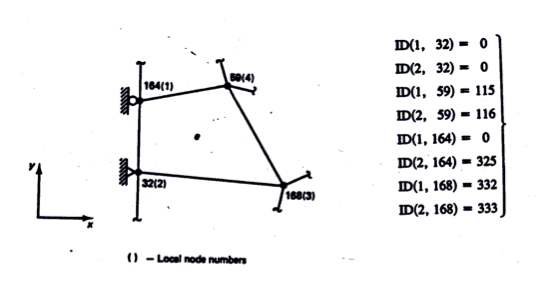
\includegraphics{images/idarraynumbering.png} 
\caption{\label{fig:idarray} An example illustrating the relationship between global nodes and equation numbers for a 2 degree of freedom problem using the id array. 
An equation number of zero denotes a boundary condition. Figure taken from Hughes, Section 3.2.}
\end{centering}
\end{figure}


With these mapping arrays, we are able to switch back and forth between looping over elements and looping over nodes. 
Global node numbering is specified by the user, and equation numbers are assigned by the code to denote the row in the stiffness matrix corresponding to the degree(s) of freedom for that node. 
One global node may have more than one equation number because there may be more than one degree of freedom per node.
Boundary conditions are specified with a zero equation number. 
Because the matrix is sparse, it is desirable to permute the stiffness matrix for computational efficiency. 
These arrays spare the user from dealing with the transformations, while making the code efficient.
Within ConMan, the data structures for these two arrays are
\begin{description}
\item [{{{{id}}}}] ( degree-of-freedom , global-node-number ) = equation-number 
\item [{{{{ien}}}}] ( local-node-number, element-number ) = global-node-number 
\item [{{{{lm}}}}] ( degree-of-freedom, local-node-number, element-number
) = global-equation-number 
\end{description}

\subsection{The Element Point of View}

Transforming between the element and global points of view is done
with the data structure called the ien array for Element to Node transformation.
The ien array takes an element number and a local node number, and
its value is the global node number. It is easiest to look at an
example.

Consider a 2-element by 2-element grid \ref{fig:smallgrid} with elements numbers consecutively in the horizontal direction and nodes numbered consecutively in the vertical direction, starting with the lower left hand corner.  For each element, the local nodes are numbered starting with the lower left-hand corner.  The ien array for this small grid is given in Table~\ref{tab:ien}.

\begin{figure}[h]
\begin{centering}
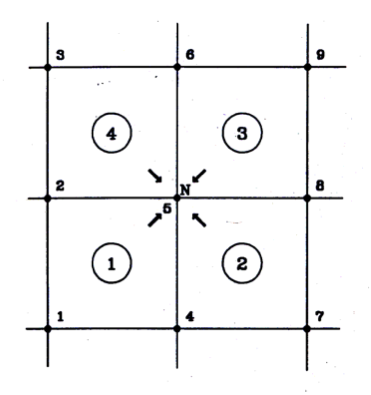
\includegraphics{images/smallgrid.png} 
\caption{\label{fig:smallgrid} An example illustrating the relationship between
global node numbers and local element numbers using the ien array.
Local nodes are numbered counterclockwise from the bottom left-hand corner.}
\end{centering}
\end{figure}

\begin{table}[h]
\centering
\begin{tabular} { l c c c c } \hline 
element & local node 1     & local node 2 & local node 3 & local node 4 \\ \hline
element 1: & ien (1, 1) = 1 & ien (1, 2) = 4 & ien (1, 3) = 5  & ien (1, 4) = 2 \\
element 2: & ien (2, 1) = 4 & ien (2, 2) = 7 & ien (2, 3) = 8  & ien (2, 4) = 5 \\
element 3: & ien (3, 1) = 5 & ien (3, 2) = 8 & ien (3, 3) = 9  & ien (3, 4) = 6 \\
element 4: & ien (4, 1) = 2 & ien (4, 2) = 5 & ien (4, 3) = 6  & ien (4, 4) = 2 \\
\hline
\end{tabular}
\caption{\label{tab:ien}ien array for the 2 element by 2 element grid shown in \ref{fig:smallgrid}.} 
\end{table}

Nodes and elements can be numbered with either the horizontal or vertical direction increasing fastest.  
This is controlled by the users choice of increment in the x and y directions for the nodes and the ien array in the \textbf{geom} file. 
For problems where flow out the left-hand side is matched by flow in the right-hand side (i.e., wrap around boundary conditions), it is necessary to increment the nodes fastest in the vertical (y) direction.
Not only does this reduce the bandwidth of the matrix, the logic of the wrap-around boundary condition assumes this ordering and will likely fail if you increment the nodes fastest in the horizontal (x) direction.

\subsection{Bousinessq Equations}

ConMan was originally written to solve the equations of creeping thermal convection using the Bousinessq approximation.   
In this version we have adapted it to include the Extended Bousinessq (EBA), Truncated Anelastic Liquid (TALA), and Anelastic Liquid (ALA) approximations.  
For brevity, we present the description of the finite element method applied to the Bousinessq approximation.

\begin{eqnarray}
\tau_{ij,j}+f_{i} & = & 0\label{eq:motion}\\
u_{i,i} & = & 0
\end{eqnarray}
where 
\begin{equation}
\tau_{ij}=-p\delta_{ij}+2\mu u_{(i,j)}
\label{eq:constit}\end{equation}
where
\begin{equation}
u_{(i,j)}=(u_{i,j}+u_{j,i})/2
\end{equation}
We replace Equation~\ref{eq:constit} with the following relationships
\begin{eqnarray}
\tau_{ij}=-p^{\lambda}\delta_{ij}+2\mu u_{(i,j)}\label{eq:constit-lam}\\
0=u_{i,i}+p^{\lambda}/\lambda.
\label{eq:constit-lam2}\end{eqnarray}
As $\lambda$ approaches infinity, these relations approach the incompressible solution. 
Also, as $\lambda$ approaches infinity, $p^{\lambda}$
approaches the hydrostatic pressure in the incompressible case. In
general, the hydrostatic pressure is $-\tau_{ii}/3$. Substituting
Equation~\ref{eq:constit-lam2} into~\ref{eq:constit-lam} we get
\begin{equation}
\tau_{ij}=\lambda u_{i,i}\delta_{ij}+2\mu u_{(i,j)}\label{eq:constit-lam-final}
\end{equation}
or 
\begin{equation}
\tau_{ii}=3\lambda u_{i,i}+2\mu u_{i,i}
\end{equation}
or 
\begin{equation}
\tau_{ii}/3=-p=(\lambda+2/3\mu)u_{i,i}
\end{equation}
but we also have 
\begin{equation}
-p^{\lambda}=\lambda u_{i,i}
\end{equation}
from Equation~\ref{eq:constit-lam2}. Clearly in the incompressible
limit $\lambda\gg\mu$ then $\lambda+2/3\mu\rightarrow\lambda$ and
$p^{\lambda}\rightarrow p$. Also note that the continuity equation
is satisfied.

Now, substituting Equation~\ref{eq:constit-lam-final} into Equation~\ref{eq:motion}
we have 
\begin{equation}
\{\lambda u_{i,i}\delta_{ij}+2\mu u_{(i,j)}\},j+f_{i}=0
\end{equation}
 At this point, it is probably easier to switch to differential notation.
These will also specialize to 2D: \begin{eqnarray}
\frac{\partial}{\partial x}\{\lambda(\frac{\partial u}{\partial x}+\frac{\partial v}{\partial y})+2\mu(\frac{\partial u}{\partial x}+\frac{\partial u}{\partial x})/2\}+\frac{\partial}{\partial y}\{2\mu(\frac{\partial v}{\partial x}+\frac{\partial u}{\partial y})/2\}+f_{x}=0\\
\frac{\partial}{\partial x}\{2\mu(\frac{\partial u}{\partial y}+\frac{\partial v}{\partial x})/2\}+\frac{\partial}{\partial y}\{\lambda(\frac{\partial u}{\partial x}+\frac{\partial v}{\partial y})+2\mu(\frac{\partial v}{\partial y}+\frac{\partial v}{\partial y})/2\}+f_{y}=0\end{eqnarray}


These are second order partial differential equations. Simplifying,
we get \begin{eqnarray}
\lambda(\frac{\partial^{2}u}{\partial x^{2}}+\frac{\partial^{2}v}{\partial x\partial y})+2\mu\frac{\partial^{2}u}{\partial x^{2}}+\mu(\frac{\partial^{2}u}{\partial y^{2}}+\frac{\partial^{2}v}{\partial y\partial x})+f_{x}=0\\
\lambda(\frac{\partial^{2}u}{\partial y\partial x}+\frac{\partial^{2}v}{\partial y^{2}})+\mu(\frac{\partial^{2}u}{\partial x\partial y}+\frac{\partial^{2}v}{\partial x^{2}})+2\mu\frac{\partial^{2}v}{\partial y^{2}}+f_{y}=0\end{eqnarray}


Now we use the same technique (approach) as we used in Possion's equation to turn the differential form into an integral form. You can either look at it as we find the variational form of the Stokes equation (which is what we are doing) or you can think of it as multiplying by a weighting function $w$ and integrating over the domain. 
Then
using integration by parts to convert the second derivatives to first
derivatives. This is done carefully by Hughes in \emph{The Finite
Element Method} on pages 197-200, but he has left out a number of
intermediate steps. Nothing about this step is hard, just tedious.
There is, however, a clever shortcut. If we return to the messy equations
at the top of the page, multiply them by the weighting function $w$
and integrate over the domain, then we do not have to use integration
by parts. To see this for yourself, simply take the equations directly
above this paragraph, multiply by a weighting function $w$ and integrate
over the 2D domain $\Omega$, then use integration by parts. You will
find (after a little algebra)

\begin{eqnarray}
\int\int_{\Omega}\frac{\partial w}{\partial x}\{\lambda(\frac{\partial u}{\partial x}+\frac{\partial v}{\partial y})+2\mu\frac{\partial u}{\partial x}\}+\frac{\partial w}{\partial y}\{2\mu(\frac{\partial v}{\partial x}+\frac{\partial u}{\partial y})/2\}\, d\Omega+\nonumber \\
\int\int_{\Omega}f_{x}\, w\, d\Omega=b.c.~terms\\
\int\int_{\Omega}\frac{\partial w}{\partial x}\{2\mu(\frac{\partial u}{\partial y}+\frac{\partial v}{\partial x})/2\}+\frac{\partial w}{\partial y}\{\lambda(\frac{\partial u}{\partial x}+\frac{\partial v}{\partial y})+2\mu\frac{\partial v}{\partial y}\}\, d\Omega+\nonumber \\
\int\int_{\Omega}f_{z}\, w\, d\Omega=b.c.~terms\end{eqnarray}
 Note that we don't get something for nothing; this shortcut does
not give us the boundary condition terms (velocity or flux). These
would fall out of the integration by parts. Recall, 
\begin{equation}
\int_{a}^{b}w\, dv=w\, v|_{a}^{b}-\int_{a}^{b}v\, dw
\end{equation}
where in our case $w$ is the weighting function and $v$ is the
second derivative term. 
The first term gives us the flux (first derivative)
boundary conditions. In the case of the momentum equations, that is
the applied tractions (or stress boundary conditions).

Now we make use of Galerkin's approximation, or more simply, we use
the same weighting functions as we use for interpolation function,
i.e., the shape functions, N. So we substitute 
\begin{eqnarray}
\frac{\partial w}{\partial x}=N_{x}\\
\frac{\partial w}{\partial y}=N_{y}\\
\frac{\partial u}{\partial x}=u\, N_{x}\\
\frac{\partial u}{\partial y}=u\, N_{y}\\
\frac{\partial v}{\partial x}=v\, N_{x}\\
\frac{\partial v}{\partial y}=v\, N_{y}
\end{eqnarray}
into our weak form equations. Although messy, that is straight-forward.
\begin{eqnarray}
\int\int_{\Omega}N_{x}\{\lambda(u\, N_{x}+v\, N_{y})+2\mu u\, N_{x}\}+N_{y}\{\mu(v\, N_{x}+u\, N_{y})\}\, d\Omega+\nonumber \\
\int\int_{\Omega}f_{x}\, w\, d\Omega=b.c.~terms\\
\int\int_{\Omega}N_{x}\{\mu(u\, N_{y}+v\, N_{x})\}+N_{y}\{\lambda(u\, N_{x}+v\, N_{y})+2\mu v\, N_{y}\}\, d\Omega+\nonumber \\
\int\int_{\Omega}f_{y}\, w\, d\Omega=b.c.~terms
\end{eqnarray}

At this point, it is useful to separate the equations into a $\lambda$
part and a $\mu$ part. We can also write them as a 2D matrix equation
\begin{equation}
[K_{\lambda}]=\left[\begin{array}{cc}
N_{x}\lambda N_{x} & N_{x}\lambda N_{z}\\
N_{z}\lambda N_{x} & N_{z}\lambda N_{z}\end{array}\right]\label{eq:Klambda}
\end{equation}
and 
\begin{equation}
[K_{\mu}]=\left[\begin{array}{cc}
N_{x}2\mu N_{x}+N_{z}\mu N_{z} & N_{z}\mu N_{x}\\
N_{x}\mu N_{z} & N_{z}2\mu N_{z}+N_{x}\mu N_{x}\end{array}\right].\label{eq:Kmu}
\end{equation}

Hughes makes use of an interesting and important observation. This
observation will greatly simplify constructing the stiffness matrix
for arbitrary coordinate systems. We can rewrite the stiffness matrices
above in the following form: \begin{equation}
[K_{\lambda}]+[K_{\mu}]=[B]^{T}[D][B]\label{eq:84}\end{equation}
 \begin{equation}
[D_{\lambda}]+[D_{\mu}]=[D]\end{equation}
 where \begin{equation}
[D_{\mu}]=\mu\left[\begin{array}{ccc}
2 & 0 & 0\\
0 & 2 & 0\\
0 & 0 & 1\end{array}\right]\end{equation}
 and \begin{equation}
[D_{\lambda}]=\lambda\left[\begin{array}{ccc}
1 & 1 & 0\\
1 & 1 & 0\\
0 & 0 & 0\end{array}\right]\end{equation}
 and \begin{equation}
[B]=\left[\begin{array}{cc}
N_{x} & 0\\
0 & N_{y}\\
N_{y} & N_{x}\end{array}\right].\end{equation}


The momentum and energy equations form a simple coupled system of
differential equations. We treat the incompressibility equation as
a constraint on the momentum equation and enforce incompressibility
in the solution of the momentum equation using a penalty formulation
described below. Since the temperatures provide the buoyancy (body
force) to drive the momentum equation and since there is no time-dependence
in the momentum equation, the algorithm to solve the system is a simple
one: Given an initial temperature field, calculate the resulting velocity
field. Use the velocities to advect the temperatures for the next
time step and solve for a new temperature field. If the time stepping
for the temperature equation is stable, then this method is stable
and converges as $\Delta t\rightarrow0$.

The element stiffness matrix (Equation~\ref{eq:84}) is made up of
the two terms from the left hand side of the integral equation. The
full element stiffness matrix for the quadralilateral element is an
8 by 8 matrix made up of 16 of the 2 by 2 matrices.
In older versions of ConMan we only stored the upper triangular part of the matrix.
{\bf New to Version 3.0:} In the original version of ConMan, we took advantage of this by considering only the upper triangular part of the stiffness matrix and saving both storage and operations using Cholesky factorization. 
In the TALA and ALA the stiffness matrix is no longer symmetric, so we now use sparse matrix factor {\bf unfact} and back substitution {\bf unback} routines for all cases.  
The integration is done using two by two Gauss quadrature, which is exact when the elements are rectangular and bilinear shape functions are used. 
The $\lambda$ term is under-integrated (one point rule) to keep the large penalty value from effectively locking the element \citep{malkus78}. 
The right-hand side is made up of three known parts, the body force term ($f_{i}$), the applied tractions ($h_{i}$) and the applied velocities ($g_{i}$).
The momentum equation is equivalent to an incompressible elastic problem, and the resulting stiffness matrix will always be positive definite \citep[p. 84-89]{hughes87}. 
More details of the method and a formal error analysis can be found in \citet{hughes79b}.
The stiffness matrix is formed in routine \textbf{f\_vstf} and the right-hand side is formed in routine \textbf{f\_tres}.

The energy equation is an advection-diffusion equation. The formal
statement is

Find $T:\Omega\rightarrow R$ such that

\begin{equation}
\dot{T}+u_{i}T_{,i}=\kappa T_{,ii}+H\,\,\,\,\,\, on\,\,\Omega
\end{equation}

\begin{equation}
T=b\,\,\,\,\,\, on\,\,\Gamma_{b}
\end{equation}

\begin{equation}
T_{,j}n_{j}=q\,\,\,\,\,\, on\,\,\Gamma_{q}
\end{equation}

\noindent where $T$ is the temperature, $u_{i}$ is the velocity,
$\kappa$ is the thermal diffusivity and $H$ is the internal heat
source. The weak form of the energy equation is given by

\begin{equation}
\int_{\Omega}\left(w+p\right)\dot{T}d\Omega=-\int_{\Omega}\left(w+p\right)\left(u_{i}T_{,i}\right)d\Omega
\end{equation}

\begin{equation}
-\kappa\int_{\Omega}w_{,i}T_{,i}d\Omega+\int_{\Gamma_{q}}wT_{,j}n_{j}d\Gamma_{q}
\end{equation}

\noindent where $\dot{T}$ is the time derivative of temperature,
$T_{,i}$ is the gradient of temperature, $w$ is the standard weighting
function and $\left(w+p\right)$ is the Petrov-Galerkin weighting
function with p, the discontinuous streamline upwind part of the Petrov-Galerkin
weighting function, given by

\begin{equation}
p=\tau u\nabla T=\tilde{k}\frac{u_{i}w_{,i}}{||u||^{2}}
\end{equation}

The energy equation is solved using Petrov-Galerkin weighting functions
on the internal heat source and advective terms to correct for the
under-diffusion and remove the oscillations which would result from
the standard Galerkin method for an advection dominated problem \citep{hughes79b}.
The Petrov-Galerkin function can be thought of as a standard Galerkin
method in which we counterbalance the numerical under diffusion by
adding an artificial diffusivity of the form
\begin{equation}
\left(\xi u_{\xi}h_{\xi}+\eta u_{\eta}h_{\eta}\right)/2
\end{equation}
\noindent with
\begin{equation}
\xi=1-\frac{2\kappa}{u_{\xi}h_{\xi}}
\end{equation}

\begin{equation}
\eta=1-\frac{2\kappa}{u_{\eta}h_{\eta}}
\end{equation}
\noindent where $h_{\xi}$ and $h_{\eta}$ are the element lengths
and $u_{\xi}$ and $u_{\eta}$ are the velocities in the local element
coordinate system ($\xi$ $\eta$ system) evaluated at the element
center. This form of discretization has no crosswind diffusion because
the {}``artificial diffusion'' acts only in the direction of the
flow (i.e., it follows the streamline), hence the name Streamline
Upwind Petrov-Galerkin (SUPG). This makes it a better approximation
than straight upwinding, and it has been demonstrated to be more accurate
than Galerkin or straight upwinding in advection dominated problems
\cite{hughes79a}. 
It has since been shown that the SUPG method is one of a broader class of methods for advection-diffusion equations referred to as Galerkin/Least-Squares methods \citep{hughes88}.

The resulting matrix equation is not symmetric, but since the energy
equation only has one degree of freedom per node, while the momentum
equation has two or three, the storage for the energy equation is
small compared to the momentum equation. 

For the explicit time stepping method, the energy equation is not implemented in matrix form. The added cost of calculating the Petrov-Galerkin weighting functions is much less than the cost of using a refined grid with the Galerkin method. 
The Galerkin method requires a finer grid then the Petrov-Galerkin method to achieve stable solutions \citep{Travis90}.

For the explicit method, the time stepping in the energy equation is done using a second-order predictor-corrector algorithm. The form of the predictor-corrector algorithm is

\noindent
Predict:
\begin{equation}
T_{n+1}^{\left(0\right)}=T_{n}+\Delta t\left(1-\alpha\right)\dot{T}_{n}
\end{equation}

\begin{equation}
\dot{T}_{n=1}^{\left(0\right)}=0
\end{equation}
Solve:
\begin{equation}
M^{*}\Delta\dot{T}_{n+1}^{\left(i\right)}=R_{n+1}^{\left(i\right)}
\end{equation}

\begin{equation}
R_{n+1}^{\left(i\right)}=-\left[\dot{T}_{n+1}^{\left(i\right)}+u\cdot\left(T_{n+1}^{\left(i\right)}\right),x\right]\left(w+p\right)-\tilde{k}w_{,x}\left(T_{n+1}^{\left(i\right)}\right),x+\,\,\,\left(boundary\, condition\, terms\right)\label{eq:residual}\end{equation}
Correct:

\begin{equation}
T_{n+1}^{\left(i+1\right)}=T_{n+1}^{\left(i\right)}+\Delta t\alpha\dot{T}_{n+1}^{\left(i\right)}\label{eq:correct1}\end{equation}


\begin{equation}
\dot{T}_{n+1}^{\left(i+1\right)}=\dot{T}_{n+1}^{\left(i\right)}+\Delta\dot{T}_{n+1}^{\left(i\right)}
\end{equation}

\noindent where $i$ is the iteration number (for the corrector),
$n$ is the time-step number, $T$ is the temperature, $\dot{T}$
is the derivative of temperature with time, $\Delta\dot{T}$ is the
correction to the temperature derivative for the iteration, $M^{*}$
is the lumped mass matrix, $R_{n+1}^{\left(i\right)}$ is the residual
term, $\Delta t$ is the time step and $\alpha$ is a convergence
parameter. Note that in the explicit formulation $M^{*}$ is diagonal.

The time step is dynamically chosen, and corresponds to the Courant time step (the largest step that can be taken explicitly and maintain stability). 
With the appropriate choice of variables, $\alpha$ = 0.5 and two iterations, the method is second order accurate \citep[][p. 562-566]{hughes87}.

The predictor step is computed in the subroutine \textbf{time\_driver}, the residual vector, $R$, is formed in the subroutine \textbf{form\_temp\_rhs\_explicit}, the lumped mass matrix , $M^{*}$, (which is a vector) is formed in the subroutine \textbf{form\_temp\_mass\_matrix}, and the corrector step is also computed in the subroutine \textbf{form\_temp\_rhs\_explicit}.

For the implicit energy equation solver, the equations are cast in a matrix form.  The big advantage here is the use of Picard iteration, which allows the solution to quickly advance to the steady-state solution in far fewer steps. This version of the energy equation uses the routines \textbf{form\_temp\_matrix} and \textbf{form\_temp\_rhs\_implicit}. 

\chapter{Incompressible and Compressible Equations}
\label{chap:compress}

Version 3.0 of ConMan includes the Extended Bousinessq Approximation (EBA), Truncated Alelastic Liquid Approximation (TALA), and Alelastic Liquid Approximation (ALA) forms of the compressible equations \citep{king10}.  
The formulation can be changed by setting the flag (itype) on the second line of the input file.
These forms follow the derivations in \citet{king10} including the use of the Adams-Williamson equation of state. 
This was a useful analytic form for a benchmark but probably not the best form for research.  
This is provides so that users can see how to extend ConMan for their own research.  
Here we repeat section 2 of \citet{king10} with comments so that the reader can follow the implementation in the code.  
The references can be found in \citet{king10}.

Mass conservation is given by
\begin{equation}
\label{masscon1}
\frac{\partial \rho}{\partial t} + \nabla \cdot ( \rho \vec{u} ) ~=~ 0,
\end{equation}
where $ \rho $ is the density and $\vec{u} $ is the velocity
The conservation of momentum is given by
\begin{equation}
\label{eqn2}
\frac{D\rho\vec{u}}{Dt} ~=~ - \nabla P  ~+~ \nabla \cdot \tau + \rho \vec{g}
\end{equation}
where $P$ is the pressure, $\vec{g}$ is the gravity, $D/Dt$ is the material derivative, and $\tau$ is the deviatoric stress tensor given by
\begin{equation}
\tau = 2 \eta \dot{\epsilon} = \eta (\nabla \vec{u} +  \nabla \vec{u}^{~T}) - \frac{2}{3} \eta \nabla \cdot \vec{u} \delta_{ij}
\label{constit-compress}
\end{equation}
where $\eta$ is the dynamic viscosity, $\dot{\epsilon}$ is the strain-rate tensor, and $\delta_{ij}$ is the Kroneker delta.   Equation \ref{constit-compress} assumes that the bulk viscosity of the fluid is zero.
Finally, the equation of energy conservation is given by,
\begin{equation}
 \rho c_p \frac{DT}{Dt} ~-~ \alpha T \frac{DP}{Dt} ~=~ \nabla \cdot (k \nabla T) ~+~ \rho H ~+~   \phi
\label{energy1}
\end{equation}
where $T$ is the temperature, $c_p$ is the heat capacity at constant pressure, $\alpha$ is the coefficient of thermal expansion, $k$ is the thermal conductivity, $H$ is the volumetric heat production and $\phi$ is the viscous dissipation given by
\begin{equation}
\label{phi}
\phi = \frac{1}{2}~ \tau : \dot{\epsilon} = \tau_{ij} \frac{\partial u_i}{\partial x_j}.
\end{equation}

In compressible convection, there is the additional required assumption--the reference state,
\begin{equation}
T = \bar{T} + T^{\prime}
\end{equation}
\begin{equation}
P = \bar{p} + p^{\prime}
\end{equation}
\begin{equation}
\rho = \bar \rho(\bar{T}, \bar{p}) + \rho^{\prime}
\end{equation}
where the over-barred quantities are time-independent and functions of depth only.
The reference pressure is given by the hydrostatic approximation
\begin{equation}
\nabla \bar{p} = \bar{\rho} g.
\end{equation}

Using the assumption that $p^{\prime} \ll \bar{p}$, we can eliminate pressure from the energy equation (\ref{energy1}), yielding
\[
 \rho c_p \frac{DT^{\prime}}{Dt} ~=~ \nabla \cdot (k \nabla (T^{\prime}+\bar{T})) ~+~ \rho H ~+~   \phi - \rho c_p \vec{u} \cdot \nabla \bar{T}
 \]
\begin{equation}
 - \alpha (\bar{T} + T^{\prime}) \bar{\rho} g w
\label{energy2}
\end{equation}
where $\vec{u} \cdot \vec{g} = -wg$, where $w$ is the upward component of velocity.

For the reference state $(\bar{\rho}, \bar{T})$, we assume an adiabatic Adams-Williamson equation of state (Birch, 1952), where
\begin{equation}
\bar{\rho}(z) = \rho_r \exp ( \frac{\alpha_r g_r}{\gamma_r c_{p_r}} z) ~~~~,~~~~
\bar{T}(z) = T_{surf} \exp ( \frac{\alpha_r g_r}{ c_{p_r}} z)
\end{equation}
where $z$ is the depth coordinate (parallel to the direction of gravity), $\gamma_r$ is the reference value for the Gr\"uneisen parameter, $T_{surf}$ is the surface temperature, and variables with the sub-script $r$ are constant values used in defining the reference state.
From this reference state, we note that $\nabla \bar{T} = (0, -\alpha_r g_r \bar{T} / c_{p_r})$, which along with dropping terms with 
$\rho^{\prime}$ and that $c_p \approx c_{p_r}$, allows us to further simplify the energy equation (\ref{energy2}),
\begin{equation}
\bar{\rho} \bar{c}_{p_r} \frac{DT^{\prime}}{Dt} ~=~ \nabla \cdot (k \nabla (T^{\prime} + \bar{T})) ~+~ \bar{\rho} H ~+~ \phi  -  \bar{\rho} \bar{\alpha} g w T^{\prime}.
\label{energy3}
\end{equation}
The expansivity $\bar{\alpha}$ is $\frac{\alpha}{\alpha_r}$ and formally dependent on the reference state. For the purposes of the benchmark, we will assume that $\bar{\alpha}~=~1$.

\section{Equations under the Anelastic Liquid Approximation (ALA)}

We nondimensionalize the equations using the reference values for density, $\rho_r$, thermal expansivity, $\alpha_r$, temperature contrast, $\Delta T_r$, thermal conductivity, $k_r$, heat capacity, $c_{p}$, once again assuming that $c_p \approx c_{p_r}$ depth of the fluid layer, $L$, and viscosity, $\eta_r$. 
The non-dimensionalization for velocity, $u_r$, pressure, $p_r$, and time, $t_r$, become
\begin{equation}
u_r = \frac{k_r}{\rho_r c_{p} L}  ~~~~,~~~~ p_r = \frac{\eta_r k_r}{\rho_r c_{p} L^2} ~~~~,~~~~ t_r =  \frac{\rho_r c_{p} L^2}{k_r}.\label{eq:nondim}
\end{equation}

The non-dimensionalization introduces four non-dimensional numbers, the Prandtl number, $Pr$, the Mach number, $M$, the dissipation number, $Di$, and the Rayleigh number, $Ra$.
If we assume that the relative volume change due to temperature, $\alpha_r \Delta T_r \ll 1$, $M^2 Pr \ll 1$ and $Pr\rightarrow \infty$, we arrive at the Anelastic Liquid Approximation (ALA).

Under the ALA, the conservation of mass becomes
\begin{equation}
\label{masscon2}
\nabla \cdot ( \bar{\rho} \vec{u} ) ~=~ 0
\end{equation}
the conservation of momentum becomes
\begin{equation}
\label{mo2}
0 ~=~ - \nabla p^{\prime}  ~+~ \nabla \cdot \tau + Di \frac{\bar{\rho} c_{p}}{K_s \gamma_r c_{v}} p^{\prime} - Ra \bar{\rho}\bar{\alpha} \hat{g} T^{\prime} /\Delta T_r
\end{equation}
where $\hat g$ is the unit vector in the direction of gravity, $c_{v}$ is the specific heat at constant volume, $\bar{\rho}$ is now dimensionless (i.e, equation (\ref{eq:nondim}) divided by $\rho_r$) and the Rayleigh number and dissipation number are given by
\begin{equation}
Ra = \frac{\alpha_r \Delta T_r {\rho_r}^2 g_r L^3 c_{p}}{\eta_r k_r}, ~~~~ Di = \frac{\alpha_r g_r L}{c_{p}}
\end{equation}

With the assumption of constant thermal conductivity, and using the dimensionless reference states for $\bar{\rho}$ and $\bar{T}$ given by
\begin{equation}
\bar{\rho} = \rho_r \exp ( z^{\prime} Di/\gamma_r ), ~~~~~~~~{\rm and}~~~~~ \bar{T} = \frac{T_{surf}}{\Delta T_r} \exp ( z^{\prime} Di ),
\end{equation}
where $z^{\prime}$ is the dimensionless vertical coordinate.
The conservation of energy (\ref{energy3}) under the ALA becomes
\begin{equation}
\bar{\rho} c_p \frac{DT^{\prime}}{Dt} + Di \bar{\rho} \bar{\alpha} w T^{\prime} ~=~ \nabla^2 T^{\prime} ~+~ \bar{\rho} H ~+~ \phi \frac{Di}{Ra} + Di^2 \bar{T}  . 
\label{energyala}
\end{equation}
Equation (\ref{energyala}) resembles the familiar energy equation in Bousinessq convection with the addition of three terms: the viscous dissipation, $ \phi \frac{Di}{Ra}$, the work done against gravity
\begin{equation}
W = Di \bar{\rho} \bar{\alpha} w T^{\prime} 
\label{w}
\end{equation}
and a second-order term in dissipation number, $ Di^2 \bar{T} $ that arises from substituting equation (17) into the $\nabla \cdot (k \nabla \bar{T})$ term in equation \ref{energy3}. 
Because $ \bar{T} $ is independent of time and only depends on depth, this terms acts like a depth-dependent internal heat source.
The volume-averaged work done against gravity $<W>$ exactly balances the volume-averaged viscous dissipation $<\phi>$ \citep{hewitt75,zhang96,leng08}.
This is one of the measures that we use to assess the energy conservation of the codes.


It is also worth pointing out that the reference state used here fails when $T_o \rightarrow 0$, leading to the non-sensible reference temperature state $\bar{T} = 0$.  
For the ALA benchmark, equations \ref{masscon2}, \ref{mo2} and \ref{energyala} are solved.

\subsection{Equations under the Truncated Anelastic Liquid Approximation (TALA)}

For the TALA, the pressure term in the buoyancy force is ignored, in which case equation \ref{mo2} becomes
\begin{equation}
\label{tala}
0 ~=~ - \nabla p^{\prime}  ~+~ \nabla \cdot \tau - Ra \bar{\rho}\bar{\alpha} \hat{g} T^{\prime} 
\end{equation}

Some numerical methods have difficulty with equation \ref{mo2} and the TALA (equation \ref{tala}) has often been used in compressible studies \citep{jarvis80,christensen85,ita94}.
\citet{jarvis80} show that there is an imbalance between viscous dissipation and gravitational potential energy with the TALA.
\citet{leng08} demonstrate that the imbalance is caused by ignoring dynamic pressure's effects on buoyancy and can be removed using the ALA.
We further compare the difference between these formulations below.

\section{Equations under the Extended Bousinessq Approximation (EBA)}

For the EBA, the reference state changes to $\bar{\rho} = 1$ and $\bar{T} = 0$.   This leads to the first step beyond the Bousinessq approximation and is a useful check that the additional terms in the energy equation that scale with dissipation number, $Di$,  have been implemented and scale properly. 
With the further assumption that $\bar{\alpha}=1, k=1$, and $\bar{c_{p_r}} =1$, the conservation and constitutive equations become
\begin{equation}
\label{masscon3}
\nabla \cdot \vec{u}  ~=~ 0,
\end{equation}
the conservation of momentum becomes
\begin{equation}
\label{moeba}
0 ~=~ - \nabla p  ~+~ \nabla \cdot \tau - Ra \hat{g} T^{\prime} 
\end{equation}
\begin{equation}
\frac{DT^{\prime}}{Dt} + Di w (T^{\prime}+ T_o) ~=~ \nabla^2 T^{\prime} ~+~ \bar{\rho} H ~+~ \phi \frac{Di}{Ra} . 
\label{energyeba}
\end{equation}
and
\begin{equation}
\label{constitba}
\tau = 2 \eta \dot{\epsilon} = \eta (\nabla \vec{u} +  \nabla \vec{u}^{~T}).
\end{equation}

Note that because $\bar{T} = 0$, the boundary condition at the base of the fluid layer remains unmodified in the EBA (i.e., $T^{\prime} = 1$).

\section{Equations under the Bousinessq Approximation (BA)}

By dropping the terms that scale with the dissipation number, $Di$, equations \ref{masscon3}-\ref{energyeba} reduce to the Bousinessq approximation.
Under the BA, equations \ref{masscon3}, \ref{moeba} and \ref{constitba} remain unchanged and equation \ref{energyeba} becomes
\begin{equation}
\frac{DT^{\prime}}{Dt}  ~=~ \nabla^2 T^{\prime} ~+~ \bar{\rho} H . 
\label{energyba}
\end{equation}

\chapter{Implementation}

\section{Introduction}

There are generally three phases to ConMan, input, time stepping, and output.
The main program is found in \textbf{ConMan.F}. 
The input is read in the files \textbf{input.F and elminp.F}. Time stepping is doing
in \textbf{time\_driver.F}. 
All output subroutines have been gathered into a subroutine called \textbf{output}.  
The rather cumbersome structure of \textbf{eglib} calling \textbf{eg2.F} for element routines has been removed.
This was originally in place to allow for different types of elements to be considered but has never been used.

In version 3.0 we have made a number of minor changes:
\begin{enumerate}
    \item Many subroutines were renamed to take advantage of the relaxation of the eight character naming limit in FORTRAN77. The major elemenr subroutines are now named \textbf{form\_velocity\_stiffness\_matrix}, \textbf{form\_velocity\_rhs}, \textbf{form\_temperature\_rhs\_explicit}, \textbf{form\_temperature\_rhs\_implicit} and the files are given the same names as the subroutines.  This should make it easier for users to follow the code.

    \item For compressible convection, the stiffness matrix is no longer symmetric, thus we now calculate the full local and global stiffness matrices and use subroutines \textbf{unfact.F} and \textbf{unback.F} to calculate the forward reduction and back substitution of the global stiffness matrix. This is not as efficient for the Bousinessq and Extended Bousinessq cases but it simplifies the code.

    \item We have removed the memory manager and now use FORTRAN's allocate function to dynamically allocate memory.  This greatly improves the portability of the code.

    \item Picard iteration is now a runtime, as opposed to compile, option.

    \item We have collected the output subroutines into a subroutine called \textbf{output.F} and this is called at the end of the time-stepping loop in subroutine \textbf{time\_drive.F}.

\end{enumerate}

\section{Material Properties}

\subsection{Buoyancy}
As discussed above, the equations in dimensionless form have one dimensionless
parameter, the Rayleigh number

\begin{equation}
Ra=\frac{g\alpha\Delta Td^{3}}{\kappa\mu}\label{eq:grav}\end{equation}

\noindent
where $g$ is the acceleration due to gravity, $\alpha$ is the coefficient
of thermal expansion, $\Delta T$ is the temperature drop across the
box, $d$ is the depth of the box, $\kappa$ is the thermal diffusivity,
and $\mu$ is the dynamic viscosity. In ConMan, the input parameter
is the buoyancy part of the Rayleigh number,

\begin{equation}
Ra_{buoy}=g\alpha\label{eq:Ra}
\end{equation}

The depth, $d$, and the temperature difference, $\Delta T$ are specified from the grid and the temperature boundary conditions, while $\kappa$ and $\mu$ are separate input parameters. 
If the depth, temperature difference, $\kappa$ and $\mu$ are set to 1, then the buoyancy number, $RA_{buoy}$, and the Rayleigh number, $Ra$, are the same.
This is the way most users set up problems in ConMan.

\subsection{Rheology}

The viscosity can be a function of temperature, pressure, or strain-rate. 
This is done in the subroutine \textbf{rheol}. 
The subroutine \textbf{rheol} is called for each element and the values of the coordinates \textit{xl}, velocity \textit{vl}, temperature \textit{tl}, and element number \textit{iel}, are passed into subroutine \textbf{rheol}. 
The viscosity, calculated at each integration point, \textit{evisc(intp)} is returned by \textbf{rheol}.
The functional form of the viscosity law depends on the choice of the input parameter \textit{ntimvs}.
If \textit{ntimvs} = 0, then a constant viscosity is used and \textit{evisc(intp)}=1.0 for each integration point.
If \textit{ntimvs} = 1, then the viscosity is a function of temperature following
\begin{equation}
    evisc(intp) = \mu_o \exp \left [ -b ~ tq(intp) \right ]
\end{equation}
where $b = 6.907755279$, $tq(intp)$,  is the temperature at the integration point (calculated from tl), and $\mu_o$ is the value of the viscosity from the input file (usually chosen to be 1.0).
The choice of $b$ gives a factor of 1000 variation across the temperature range of 0 to 1.  This is the rheology used in \citet{blankenbach89} case 2a.
If \textit{ntimvs} = 2, then the viscosity is a function of temperature following
\begin{equation}
    evisc(intp) = \mu_o \exp \left [ -b ~ tq(intp) + c \left ( 1.0-zq(intp) \right ) \right ]
\end{equation}
where $b = 9.704060528$, $c=4.148883083$, $tq(intp)$, is the temperature at the integration point (calculated from tl), $\left ( 1.0 - zq(intp) \right )$ is the depth of the domain and $\mu_o$ is the value of the viscosity from the input file (usually chosen to be 1.0).
The choice of $b$ gives a factor of 10000 variation across the temperature range of 0 to 1.  
This is the rheology used in \citet{blankenbach89} case 2b.

If \textit{ntimvs} = 3, then the viscosity is a function of temperature and pressure following an Arrhenius formulation,
\begin{equation}
evisc(intp) =\mu_{o}\left\{ \exp\left\{ \frac{E^{*}*1.0e3+V^{*}(1.0-z(intp))}
{R*(tq(intp)+T_{o})}\right\} -\exp\left\{ \frac{E^{*}*1.0e3+V^{*}(1.0-z(intp)}{R*(1+T_{o})}\right\} \right\} \label{eq:munew}
\end{equation}
where $\mu_{o}$ is the preexponential viscosity, $E^{*}$ is the activation energy (set in the input file), $V^{*}$ is the activation volume (set in the input file), and $T_{o}$ is the temperature offset.
In the input files, $\mu_{o}$, is input on the viscosity card, $E^{*}$ is input as Tcon(1), $V^{*}$ is input as Tcon(2), and $T_{o}$ is hardwired in \textbf{rheol.F} to be 273. $\Delta T$ is hardwired to be 2000.0.
The scaling in \textbf{rheol.F} is such that $E^{*}$ can be input in kJ/mole and $V^{*}$ can be input as cm$^{3}$.

If \textit{ntimvs} = 4, the rheology is a combination dislocation/diffusion creep rheology following ...

If \textit{ntimvs} = 5, the rheology is a yield-stress formulation consistent with \citet{stein08}.
In this form, the effective viscosity \textit{evisc(intp)},
\begin{equation}
    evisc(intp) = \frac{2}{ \frac{1}{\eta_{PT}} + \frac{1}{\eta_E}}
\end{equation}
where $\eta_{pT}$ is the pressure and temperature dependent rheology,
\begin{equation}
    \eta_{PT} = \exp \left [ -b ~ tl(intp) + c ( 1-z(intp) ) \right ]
\end{equation}
and $\eta_E$, is the viscoplastic form
\begin{equation}
    \eta_{E} = \eta^* + \frac{\sigma_y}{\dot{e}_2}
\end{equation}
where $\eta^*$ is the plastic rheology, $\sigma_y$ is the yield stress rheology, and $\dot{e}_2$ is the second invarient of the strain-rate tensor.
In this formulation, $\eta^*$ is hard-wired to $10^{-5}$ and $b$ is hard-wired to $11.512925 = \ln 10^5$. $c$ is set from the input file (tcon(1)) and $\sigma_y$ is set from the input file (tcon(2)).

If \textit{ntimvs} = 6, the rheology is a simple Frank Kaminetskii
approximation, as above, but non-dimensionalized $b$ and $c$ constants
are now read
in when activation energy and volume cards are read ($z$ and $tq$ non-dimensional):
\begin{equation}
    \eta_{PT} = \exp \left [ -b (0.5-tq(intp)) + c ( 1-z(intp) ) \right ].
\end{equation}



The user can easily modify the existing or add new rheology options for specific problems of interest.
Using \textit{ntimvs} = 4 or 5 one should add an iteration loop within each time step in subroutine \textbf{time\_drive.F} to allow the change in velocity each step to come to consistency with the rheology.
Experience has shown that after the first step, which may require 10-20 iterations, 2-3 iterations per step is all that is needed to converge \citep{king90a}.

Users who are new to viscous flow should approach viscoplastic or composite rheologies with an abundance of caution, as small changes can cause convergence headaches and/or unexpected results.

\subsection{Internal Heating}

Internal heating can be specified through the internal heating parameter.
If no bottom temperature is specified, the Rayleigh number becomes

\begin{equation}
Ra=\frac{g\alpha Hd^{5}}{k\kappa\mu}
\end{equation}
where $H$ is the internal heating parameter and $k$ is the thermal conductivity. 
The grid can have multiple material groups, each with its own set of material properties.

\chapter{Installation}

\section{Building from Source}

\subsection{System Requirements}

ConMan has been tested on a variety of computational platforms including:

\begin{itemize}
\item Mac OS X El Capitan (10.11.6) (gfortan configured with gcc version 6.1.0) 
\item Scientific Linux 6.10 (gfortran configured with gcc version 4.4.7 20120313)
\item ubuntu xxxx (?) \em{placeholder for CIG information}
\end{itemize}

It is likely to run on other platforms as well but has not been tested.

\subsection{Dependencies}

This version of ConMan is self-contained and requires no external libraries.

\subsection{\label{sec:Downloading-the-Code}Downloading and Unpacking the ConMan
Code}

You can get the source for the latest release from the ConMan web
page \url{geodynamics.org/cig/software/packages/mc/conman/}. Download
the source archive and unpack it using the \texttt{tar} command:

\begin{lyxcode}
\$~tar~xzf~ConMan-3.0.tar.gz
\end{lyxcode}
Advanced users and software developers may be interested in downloading the latest ConMan source code directly from the CIG source code repository, instead of using the prepared source package. 
To check whether you have the git version control client installed on your machine, type:

\begin{lyxcode}
git --version
\end{lyxcode}
You should get a response that looks something like this:

\begin{lyxcode}
git version 2.8.4 (Apple Git-73
\end{lyxcode}
Otherwise, you will need to download and install git,
available at the Git Website \url{https://git-scm.com/downloads}.
Then the code can be checked out with the following command:

\begin{lyxcode}
git~clone~https://github.com/geodynamics/conman.git
\end{lyxcode}
The ConMan software package contains the follow directories:

\begin{description}
\item [{\textasciitilde{}/src}] ConMan source code directory.
\item [{\textasciitilde{}/doc}] ConMan manual and other documentation.
\item [{\textasciitilde{}/cookbook1}] input and geometry files for the
Blankenbach benchmark cases.
\item [{\textasciitilde{}/cookbook2}] input and geometry files for the
driven slab problem in \citet{vanKeken08}.
\item [{\textasciitilde{}/cookbook3}] input and geometry files for the
compressible benchmarks in \citet{king10}.
\end{description}

\subsection{Compiling and Running ConMan}

ConMan comes ready to run with a standard \textbf{Makefile} that contains the system calls for the compiler (FC) and the loader (LD). 
The distribution assumes this is gfortran, otherwise they will need to be modified for your local environment. 

There are no external libraries or packages required. 
All source code is in the directories src, src/grid.src, src/utils.src, and src/solver.src

Typing `make' in the src directory will produce the ConMan executable \texttt{conman} in the main directory. 
The warning messages {\em Branch at (1) may result in an infinite loop} are normal and expected.
We take advantage of FORTRAN's ability to continue reading a file after a read error.
This is done to allow the user to annotate files with comments, which has proven to be a useful and popular feature.
If there is really and input error, the code will fail and ususally the problem can be diagonsed looking at the file \textbf{out.xxxx}.

To run ConMan type:
\begin{lyxcode}
\$~conman~<~runfile
\end{lyxcode}
where \texttt{runfile} is a text file that has a list of filenames
that can be up to 80 characters long. For more details on \texttt{runfile},
see Chapter \ref{cha:Output-Guide}.

\section{\label{sec:Support}Support}

The primary point of support for ConMan is the CIG Mantle Convection
Mailing List \url{cig-mc@geodynamics.org}. Feel free to send questions,
comments, feature requests, and bugs to the list. The mailing list
is archived at

\begin{lyxcode}
cig-mc~Archives~\url{geodynamics.org/pipermail/cig-mc/}


\end{lyxcode}

{\em WE DO NOT USE ROUNDUP ANY LONGER}

You may also use the bug tracker

\begin{lyxcode}
Roundup~\url{geodynamics.org/roundup}
\end{lyxcode}
to submit bugs and requests for new features.

{\em FEATURE REQUESTS SHOULD GO TO ISSUES. BUGS TOO???}

\chapter{\label{cha:Input-Guide}Input Guide}

To run ConMan a series of nine file names are needed, some for input and some for output. Usually these are read from a runfile. 
The first two files are input files \textbf{input} and \textbf{geom} and are described in this section. The third file is an output file showing all the input parameters in a verbose form. 
The fourth and fifth files are an input temperature file (optional) and an output temperature file. 
These are for starting a new run from a previous run. The sixth file is a time series file (see routine \textbf{fluxke}), the seventh file is the coordinates, velocities and temperatures, the eighth file
is for stresses (see routine \textbf{stress.F}) and the ninth file is for geoid and topography (see routine \textbf{geoid.F}). 
These file names are read in subroutine \textbf{ConMan.F}.

The input for ConMan is read from two different FORTRAN units. 
The first unit, \textbf{iin}, contains the time stepping, output, and material parameters as well as element type information while the second unit, \textbf{igeom}, contains the coordinates, boundary values and connectivity information. 
ConMan reads the file names to attach to these units from standard input. 
The typical way to run ConMan is to create a file with nine lines, one file name per line, and redirect this into the executable (i.e., \% conman.pic < runfile \& ). \textbf{iin}
is attached to the file named on the first line and \textbf{igeom}
is attached to the file named on the second line (names must be ASCII
with a length less than 80 characters long).

The input deck was broken up so that an automatic grid generating
routine could be used to generate coordinates, boundary conditions
and element connectivities separate from ConMan. The only automatic
grid generation ConMan does is linear or bilinear interpolation which
is described in the appropriate sections of this guide.

The following sixteen cards or groups of cards are read from the \textbf{iin}
unit (throughout this guide a {}``card'' will mean one line of an
ASCII text file). These constitute the parameter part of the input
{}``deck'' for the program ConMan. The format for this guide is
a \textbf{bold} title line giving the card title followed by an \emph{italicized}
line showing the order of the parameters and a listing of the parameters
(with a brief explanation).

\section{General Input File}

\begin{description}
\item [{{{{Title~Card}}}}] \emph{Any descriptive character string
up to 80 characters long} 
\item [{{{{Global~Constants~Card}}}}] \emph{numnp nsd ndof nelx
nelz mprec iflow necho inrsts iorstr nodebn ntimvs ntseq numeg isky
nwrap}

\begin{description}
\item [{{{{numnp}}}}] . . . . . . total number of nodal points (integer)
\item [{{{{nelx}}}}] . . . . . . . number of elements in the x1 (horizontal) (integer)
direction 
\item [{{{{nelz}}}}] . . . . . . . number of elements in the x2 (vertical) (integer)
direction 

\item [{{{{iflow}}}}] . . . . . . . data check flag (integer)


0 - check data only

1 - execute code

\item [{{{{necho}}}}] . . . . . . echo data flag (integer)


0 - minimum data echo (terse)

1 - echo data to output file (verbose)

\item [{{{{inrstr}}}}] . . . . . . . read restart file flag (integer)


0 - use default start (conductive)

1 - read restart file from unit 16

\item [{{{{iorstr}}}}] . . . . . . . write restart file flag (integer)


0 - don\textquoteright{}t write restart file

1 - write restart file to unit 17

\item [{{{{nodebn}}}}] . . . . . . number of edge nodes for nusselt (integer)
smoother 
\item [{{{{ntimvs}}}}] . . . . . . temperature dependent viscosity (integer)
flag


0 - stiffness matrix factored once -- constant viscosity

1 - Blankenbach 2a case (hardwired constants)

2 - Blankenbach 2b case (hardwired constants)

3 - temperature dependent Arrhenius law (diffusion creep) using activation energy and volume below

4 - composite dislocation/diffusion creep (code does not currently support non-Newtonian dislocation creep)

5 - rheology based on Stein and Hansen (20xx?) (currently code does not currently support non-Newtonian dislocation creep)

6 - Frank-Kaminetskii with variable constants

\item [{{{{nwrap}}}}] . . . . . . number of nodes to wrap (integer)


equal to number of elements in vertical (this requires nodes must be 

numbered increasing fastest in vertical direction)

\item [{{{{itype}}}}] . . . . . . compressible formulation (integer)

1 - ALA

2 - TALA

3 - EBA

4 - BA

5 - subduction benchmark, wedge test, use BA

6 - subduction benchmark, wedge test, interpret tmovis as $v_p$ for Batchelor, use BA

\item [{{{{isolve}}}}] . . . . . .  temperature solver (integer)

1 - explicit

2 - implicit

3 - Picard

\end{description}

\end{description}

\begin{description}
\item [{{{{Time~Sequence~Card}}}}] \emph{nstep accel}

\begin{description}
\item [{{{{nstep}}}}] . . . . . . . number of time steps (integer)
\item [{{{{accel}}}}] . . . . . . . a factor that multiplies the time step (real number)
\end{description}

\item [{{{{Output~Step~Card}}}}] \emph{nstprt tmax datasv tsave tmovie }

\begin{description}
\item [{{{{nstprt}}}}] . . . . . . steps between output (integer)
\item [{{{{tmax}}}}] . . . . . . . maximum time, usually diffusion scaling (real)
\item [{{{{datasv}}}}] . . . . . . time interval for time series output (real)
\item [{{{{tsave}}}}]. . . . . . . time interval for temperature/velocity output (real)
\item [{{{{tmovis}}}}] . . . . . . time interval for movie output (real) - not supported
\end{description}

\item [{{{{Velocity~Boundary~Condition~Flag~Cards}}}}] \emph{bnode enode incr (bcf(i), i=1,ndof)}

\begin{description}
\item [{{{{bnode}}}}] . . . . . . beginning node 
\item [{{{{enode}}}}] . . . . . . ending node 
\item [{{{{incr}}}}] . . . . . . . node increment 
\item [{{{{bcf(i)}}}}]. . . . . . boundary condition flag for ith degree of freedom

0 - free slip

1 - pinned degree of freedom

2 - Batchelor (corner flow) solution

\end{description}

\emph{0 0 0 0 0 to end VBCF cards}

\item [{{{{Temperature~Boundary~Condition~Flag~Cards}}}}] \emph{bnode enode incr bcf}

\begin{description}
\item [{{{{bnode}}}}] . . . . . . beginning node 
\item [{{{{enode}}}}] . . . . . . ending node 
\item [{{{{incr~}}}}] . . . . . . node increment 
\item [{{{{bcf~~}}}}] . . . . . . boundary condition flag for temperature

1- fixed temperature

\end{description}
\emph{0 0 0 0 to end TBCF cards}

\item [{{{{Nusselt~Number~Boundary~Condition~Flag~Cards~-~Edge~Nodes}}}}] top
and bottom rows of nodes \emph{bnode enode incr}

\begin{description}
\item [{{{{bnode}}}}] . . . . . . beginning node 
\item [{{{{enode}}}}] . . . . . . ending node 
\item [{{{{incr~}}}}] . . . . . . node increment 
\end{description}
\emph{0 0 0 to end NNBCF (type a) cards}

\item [{{{{Nusselt~Number~Boundary~Condition~Flag~Cards~-~Second~Row~Nodes}}}}] second
from top and bottom rows of nodes \emph{bnode enode incr}

\begin{description}
\item [{{{{bnode}}}}] . . . . . . beginning node 
\item [{{{{enode}}}}] . . . . . . ending node 
\item [{{{{incr~}}}}] . . . . . . node increment 
\end{description}
\emph{0 0 0 to end NNBCF (type b) cards}

\item [{{{{Initial~Temperature~Card}}}}] \emph{pert xsize zsize}

\begin{description}
\item [{{{{pert~}}}}] . . . . . . . perturbation from conductive state 
\item [{{{{xsize}}}}] . . . . . . . nondimensional length (x1 direction)
of box 
\item [{{{{zsize}}}}] . . . . . . . nondimensional height (x2 direction)
of box 
\end{description}
\item [{{{{Equation~of~state~Card}}}}] \emph{Di T0 diff\_T cgamma rho0}

\begin{description}
\item [{{{{Di~~~}}}}] . . . . . . . Dissipation number 
\item [{{{{T0~~~}}}}] . . . . . . . surface temperature (dimensional)
\item [{{{{diff\_T}}}}] . . . . . . . temperature difference across the box (dimensional)
\item [{{{{cgamma}}}}] . . . . . . . Gruneisen parameter (non-dimensional)
\item [{{{{rho0~}}}}] . . . . . . . reference density (non-dimensional)
\end{description}

\item [{{{{Element~Parameter~Card}}}}] - \emph{numat numsuf}

\begin{description} 
\item [{{{{numat~}}}}]. . . . . . number of material groups 
\item [{{{{numsuf}}}}]. . . . . . number of imposed stress/flux cards 
\end{description}
\item [{{{{Viscosity~Card}}}}] \emph{visc(i), i=1,numat}

\begin{description}
\item [{{{{visc(i)}}}}] . . . . . . preexponential viscosity coefficient for ith material group 
\end{description}
\item [{{{{Penalty~Card}}}}] \emph{alam(i), i=1,numat}

\begin{description}
\item [{{{{alam(i)}}}}] . . . . . . penalty parameter for ith material group 
\end{description}
\item [{{{{Diffusivity~Card}}}}] \emph{diff(i), i=1,numat}

\begin{description}
\item [{{{{diff(i)}}}}] . . . . . . . thermal diffusivity for ith material group 
\end{description}
\item [{{{{Buoyancy~Rayleigh~Number~Card}}}}] \emph{Ra(i), i=1,numat}

\begin{description}
\item [{{{{Ra(i)}}}}] . . . . . . . bouyancy part of Rayleigh number for ith material group 
\end{description}
\item [{{{{Internal~Heating~Parameter~Card}}}}] \emph{dmhu(i), i=1,numat}

\begin{description}
\item [{{{{dmhu(i)}}}}] . . . . . . internal heat source for ith material group 
\end{description}
\item [{{{{Activation~Energy~Card}}}}] \emph{tcon(1,i), i=1,numat}

\begin{description}
\item [{{{{tcon(1,i)}}}}] . . . . . activation energy for ith material group for temperature dependent viscosity (kJ/mole) 
\end{description}
\item [{{{{Activation~Volume~Card}}}}] \emph{tcon(2,i), i=1,numat}

\begin{description}
\item [{{{{tcon(2,i)}}}}] . . . . . activation volume for ith material group for temperature dependent viscosity (cm$^{3}$/mole) 
\end{description}
\item [{{{{Viscosity~Cutoff~Card}}}}] \emph{tcon(3,i), i=1,numat}


\item [{{{{Surface~Force/Flux~Cards}}}}] - numsuf cards \emph{nel side fnorm ftan flux}

\begin{description}
\item [{{{{nel}}}}] . . . . . . . . element number 
\item [{{{{side}}}}] . . . . . . . side to apply force and flux

1 - bottom

2 - right side

3 - top

4 - left side

\item [{{{{fnorm}}}}] . . . . . . . normal surface force 
\item [{{{{ftan}}}}] . . . . . . . tangential surface force 
\item [{{{{flux}}}}] . . . . . . . . heat flux 
\end{description}
\end{description}
The following four groups of cards are read from the \textbf{igeom}
unit. These constitute the geometry part of the input {}``deck''
for the program \texttt{conman}. The format of this section is the
same as above.

\section{Geometry Input File}

\begin{description}

\item [{{{{Coordinate~Group}}}}]{~~~~}

\begin{description}
\item [{{{{Absolute~Coordinate~Card}}}}] \emph{node gp (x(i,node)
i=1,nsd)}

\begin{description}
\item [{{{{node}}}}] . . . . . . . the node whose coordinates are
to be specified 
\item [{{{{gp}}}}] . . . . . . . . generation parameter for automatic
generation

0 - no autogeneration

2 - generate a line using node as a starting point

4 - generate a box using node as the lower left corner

\item [{{{{x(i,node)}}}}] . . . . . coordinate value in the ith spatial
dimension 
\end{description}
\item [{{{{Corner~Generation~Cards}}}}] - gp-1 cards \emph{node
mgen (x(i,node) i=1,nsd)}

\begin{description}
\item [{{{{node}}}}] . . . . . . . node number 
\item [{{{{mgen}}}}] . . . . . . . generation parameter


0 - don\textquoteright{}t use this as the start of a generation
sequence

1 - use this as the start of a generation sequence

\item [{{{{x(i,node)}}}}] . . . . . coordinate value in the ith spatial
dimension 
\end{description}
\item [{{{{Generation~Increment~Card}}}}] \emph{ninc1 inc1 ninc2
inc2}

\begin{description}
\item [{{{{ninc1}}}}] . . . . . . . number of additional nodes to
generate in x1 direction 
\item [{{{{inc1}}}}] . . . . . . . increment of nodes in x1 direction 
\item [{{{{ninc2}}}}] . . . . . . . number of additional nodes to
generate in x2 direction


0 - if gp equals 2

\item [{{{{inc2}}}}] . . . . . . . increment of nodes in x2 direction


0 - if gp equals 2

\end{description}
\emph{0 0 0 0 to end coordinate group}

\end{description}

\end{description}

\begin{description}

\item[{{{Velocity Boundary Condition Group }}}] {~~~~}

\begin{description}
\item [{{{{Absolute~Velocity~Card}}}}] \emph{node gp (v(i,node)
i=1,nsd)}

\begin{description}
\item [{{{{node}}}}] . . . . . . . the node whose velocities are
to be specified 
\item [{{{{gp}}}}] . . . . . . . . generation parameter for automatic
generation


0 - no autogeneration

2 - generate a line using node as a starting point

4 - generate a box using node as the lower left corner

\item [{{{{v(i,node)}}}}] . . . . . velocity value in the ith spatial
dimension 
\end{description}
\item [{{{{Corner~Generation~Cards}}}}] - gp-1 cards \emph{node
mgen (v(i,node) i=1,nsd)}

\begin{description}
\item [{{{{node}}}}] . . . . . . . node number 
\item [{{{{mgen}}}}] . . . . . . . generation parameter


0 - don\textquoteright{}t use this as the start of a generation
sequence

1 - use this as the start of a generation sequence

\item [{{{{v(i,node)}}}}] . . . . . velocity value in the ith spatial
dimension 
\end{description}
\item [{{{{Generation~Increment~Card}}}}] \emph{ninc1 inc1 ninc2
inc2}

\begin{description}
\item [{{{{ninc1}}}}] . . . . . . . number of additional nodes to
generate in x1 direction 
\item [{{{{inc1}}}}] . . . . . . . increment of nodes in x1 direction 
\item [{{{{ninc2}}}}] . . . . . . . number of additional nodes to
generate in x2 direction

\begin{description}
\item [{{{{0}}}}] - if gp equals 2 
\end{description}
\item [{{{{inc2}}}}] . . . . . . . increment of nodes in x2 direction


0 - if gp equals 2

\end{description}
\emph{0 0 0 0 to end velocity group}

\end{description}

\end{description}

\begin{description}

\item [{{{{Temperature Boundary Condition Group }}}}]{~~~~}

\begin{description}
\item [{{{{Absolute~Temperature~Card}}}}] \emph{node gp t(node)}

\begin{description}
\item [{{{{node}}}}] . . . . . . . the node whose velocities are
to be specified 
\item [{{{{gp}}}}] . . . . . . . . generation parameter for automatic
generation


0 - no autogeneration

2 - generate a line using node as a starting point

\item [{{{{t(node)}}}}] . . . . . . temperature value 
\end{description}
\item [{{{{Corner~Generation~Cards}}}}] - gp-1 cards \emph{node
mgen t(node)}

\begin{description}
\item [{{{{node}}}}] . . . . . . . node number 
\item [{{{{mgen}}}}] . . . . . . . generation parameter


0 - don\textquoteright{}t use this as the start of a generation
sequence

1 - use this as the start of a generation sequence

\item [{{{{t(node)}}}}] . . . . . . temperature value 
\end{description}
\item [{{{{Generation~Increment~Card}}}}] \emph{ninc1 inc1 ninc2
inc2}

\begin{description}
\item [{{{{ninc1}}}}] . . . . . . . number of additional nodes to
generate in x1 direction 
\item [{{{{inc1}}}}] . . . . . . . increment of nodes in x1 direction 
\item [{{{{ninc2}}}}] . . . . . . . number of additional nodes to
generate in x2 direction


0 - if gp equals 2

\item [{{{{inc2}}}}] . . . . . . . increment of nodes in x2 direction


0 - if gp equals 2

\end{description}
\emph{0 0 to end temperature group}

\end{description}

\end{description}

\begin{description}

\item [{{{{Element Connectivity (ien) Generation Group }}}}]{~~~~}

\begin{description}
\item [{{{{Absolution~Element~Card}}}}] \emph{elnu ng mat no (ien(elnu,i)
i=1,nen)}

\begin{description}
\item [{{{{elnu}}}}] . . . . . . . element number 
\item [{{{{ng}}}}] . . . . . . . . generation parameter


0 - no generation

1 - generate using increments from increment card

\item [{{{{mat}}}}] no . . . . . . material number for this element 
\item [{{{{ien(elnu,i)}}}}] . . . . . global node number for the
ith local node of element counterclockwise from lower left corner 
\end{description}
\item [{{{{Increment~Card}}}}] \emph{nel1 incel1 incn1 nel2 incel2
incn2}

\begin{description}
\item [{{{{nel1}}}}] . . . . . . . number of elements in x1 (horizontal)
direction 
\item [{{{{incel1}}}}] . . . . . . . increment of elements in x1
(horizontal) direction 
\item [{{{{incn1}}}}] . . . . . . . increment of nodes in x1 (horizontal)
direction 
\item [{{{{nel2}}}}] . . . . . . . number of elements in x2 (vertical)
direction 
\item [{{{{incel2}}}}] . . . . . . . increment of elements in x2
(vertical) direction 
\item [{{{{incn2}}}}] . . . . . . . increment of nodes in x2 (vertical)
direction 
\end{description}
\emph{0 0 0 0 0 0 to end element connectivity group}

\end{description}

\end{description}

\chapter{\label{cha:Sample-Input-Files}Sample Input Files }

The lines below are a sample 50 element by 50 element input deck for
a 1 by 1 square, constant viscosity with the Picard method. This is
Blankenbach 1a:

\begin{lyxcode}
50~x~50~el.~plate~problem~from~Blankenbach~et~al.,~1989

~\#Nds~~~~X~~~Z~~ck~echo~rrst~wrst~nus~tdvf~~iwrap~~itype~isolve

~~2601~~50~~50~~~1~~~~0~~~~0~~~~1~102~~~~0~~~~~~0~~~~~~4~~~~~~3

~time~step~information

~~~~100~~~1~~1.0~~1.0~~0.50000

~output~information

~~~~100~~~~100~~~~100~~~~100

~velocity~boundary~condition~flags:~IFCMT,DELNXTLN

~bnode~~~enode~~~incr~bcf1~bcf2

~~~~~1~~2551~~~~~51~~~~0~~~~1

~~2551~~2601~~~~~~1~~~~1~~~~0

~~~~~~1~~~51~~~~~~1~~~~1~~~~0

~~~~51~~2601~~~~~51~~~~0~~~~1

~~~~~1~~~~~1~~~~~~1~~~~1~~~~1

~~~~51~~~~51~~~~~~1~~~~1~~~~1

~~2551~~2551~~~~~~1~~~~1~~~~1

~~2601~~2601~~~~~~1~~~~1~~~~1

~~~~~~0~~~~~~0~~~~~~0~~~~0~~~~0

~temperature~boundary~condition~flags

~~~~~1~~2551~~~~51~~~~1

~~~~51~~2601~~~~51~~~~1

~~~~~~0~~~~~~0~~~~~~0~~~~0

~bndy~info~(top~-~bottom~rows)

~~~~~1~~2551~~~~51

~~~~51~~2601~~~~51

~~~~~~0~~~~~~0~~~~~~0

~bndy~info~(2nd~from~top~-~2nd~from~bottom~rows)

~~~~~~2~~2552~~~~51

~~~~~50~~2600~~~~51

~~~~~~0~~~~~~0~~~~~~0

~initial~condition~information

~~~~0.1~~~~1.0~~~~1.0~~~~1.0

~element~information

~2~~2500~4~4~1~2~0~5~0~0

~viscosity

~~1.0e0~~

~penalty~number

~~0.1E+08~

~diffusivity~(always~one)

~~~~1.0~~~

~Rayleigh~number

~~1.0e+04~~

~internal~heating~parameter

~~~~0.0

~~~~0.0

~~~~0.0~~~

~~~~1.0e7~~~
\end{lyxcode}
The lines below are a sample geometry file for the 50 by 50 element
problem.

\begin{lyxcode}
coordinates

~~~~~~1~~~~4~~0.0~~0.0

~~~2551~~~~1~~1.0~~0.0

~~~2601~~~~1~~1.0~~1.0

~~~~~51~~~~1~~0.0~~1.0

~~~~~50~~~51~~~50~~~~1

~~~~~~0~~~~0~~0.0~~0.0

~velocity~boundary~conditions~(non-zero)

~~~~~~0~~~~0~~0.0~~0.0

~temperature~boundary~conditions~(non-zero)

~~~~~~1~~~~2~~1.0

~~~2551~~~~0~~1.0

~~~~~50~~~51

~~~~~~0~~~~0~~0.0

~element~connectivity~and~material~groups

~~~~~~1~~~~~~1~~~~~~1~~~~~~1~~~~~52~~~~~53~~~~~~2

~~~~~50~~~~~50~~~~~51~~~~~50~~~~~~1~~~~~~1

~~~~~~0~~~~~~0~~~~~~0~~~~~~0~~~~~~0~~~~~~0~~~~~~0
\end{lyxcode}

\chapter{\label{cha:Output-Guide}Output Guide}


\section{The Output Files}

The 10 required output files names are taken from the names in the runfile. The
execution of \texttt{conman} proceeds by \% conman < runfile where
the runfile has a list of filenames that can be up to 80 characters
long.

\noindent The names in the runfile are attached to the following input
or output files.

\begin{lyxcode}
input~

geometry~

output~

input~restart~

output~restart~

time~series~output~

temperature~and~velocity~field~output~

stress~and~viscosity~field~output~

compressible~benchmark~output~

geoid~output~
\end{lyxcode}
All files are ASCII files. The {\em input} and {\em geometry}
files are as described in the previous section.

The {\em output} file is a formatted record of the input. If the
variable {\em necho} is set to one, then values of the coordinates
and boundary conditions are output and the file can become large.
Near the end of the {\em output} file execution time is listed
for various subparts of the code.

The {\em restart input} file is an input file that is used if the
variable {\em inrstr} is set to one. The file is ASCII but formatted
and the format statement can be found in the file \textbf{input.F}.
The first line contains the initial timestep and time, the second
line is a header, and the third through {\em numnp} lines contains
the node, temperature and time derivative of temperature.

The {\em restart output} file is an output file that is used if
the variable {\em iorstr} is set to one. We recommend this always
be set to run. This file is overwritten every {\em nsdprt} steps
and the output is written from the file \textbf{timdrv.F}

The {\em time series output} file is written every time step. The
values are ASCII and are heat flux at the bottom, heat flux at the
top, kinetic energy, and time. All values are dimensionless. This
file is written from the routine \textbf{fluxke.F}

The {\em Temperature and velocity output} file is an ASCII file
written from the routine \textbf{print.F}. There are two header lines
that contain {\em nsd, nelx, nelz, numnp, nstep, time}. The second
line labels the output and the third through numnp lines list the
node, x, z, vx, vz, and temperature values at each node. This file
is output every {\em nsvprt} steps and each successive set of values
is appended to the end of the file. The unix command {\em split
-{numnp+2} tempfile} can be used to split the file into files that
are {\em numnp+2} lines long.

The {\em stress output} file is an ASCII file written from the
routine \textbf{prtstr} which can be found in the file \textbf{stress.F}.
Like the temperature velocity file there are two header lines that
contain {\em nsd, nelx, nelz, numnp, nstep, time}. The second line
labels the output and the third through \texttt{numnp} lines list
the node, x, z, txx, tzz. txz. p and viscosity at each node. This
file is output every {\em nsvprt} steps and each successive set
of values is appended to the end of the file. The unix command {\em
split -{numnp+2} tempfile} can be used to split the file into files
that are {\em numnp+2} lines long.

The {\em compressible benchmark output} file contains time series of output requested in the benchmark paper.  The calculations are done in \textbf{print\_compbm\_data.F} Some of the calculations are repeated from \textbf{fluxke.F} but the duplication was left in place.
Both subroutines are called in \textbf{output.F} and one or the other could be disabled if the user so chooses.

The {\em geoid output} file contains the horizontal coordinate,
the dynamic topography, the geoid contribution from the temperature
only and the total geoid (from surface and cmb topography, and internal
(i.e., temperature) density contrasts). This is written from the file
\textbf{geoid.F}. The dimensional values are hard wired into the code
and can be found at the top of \textbf{geoid.F}. This version of the
geoid code has not been tested with flow-through boundary conditions
(i.e, {\em nwrap = nelz}).
{\em \textbf{\textcolor{red}{Warning.}} As written, the code assumes the parameters from \citet{blankenbach89} and adjusts the viscosity as the Rayleigh number changes.
It would be ideal to make the scaling parameters input.
This is left to the user community.

See Table~\ref{tab:blankenbach-params}.
It is best to carefully check the \textbf{geoid.F} source for the specific problem of interest.}

The {\em geoid output} file contains additional output for the compressible case.  The columns are: Rayleigh number, Nusselt Number,
Vrms, maximum surface velocity, average surface velocity, rms temperature,
volume-average viscous dissipation, $\phi$, and 
volume-average work against the gravitational potential, $W$. 
In the ALA approximation, $\phi$ and $W$ should exactly balance.
This is a measure of the energy conservation approximation.

\chapter{\label{cha:The-Benchmark-Cases}The Benchmark Cases}

We provide input and geometry files for the benchmark cases described
below in the directories \texttt{cookbook1, cookbook2} and \texttt{cookbook3}.

\section{Cookbook 1: Blankenbach Benchmark Cases}

Here we reproduce the results from \citet{blankenbach89} for constant viscosity and temperature-dependent viscosity in a unit-aspect ratio domain, with free-slip boundary conditions, heated from below and cooled from above. 
ConMan results were not a part of the \citet{blankenbach89} paper but results from the the grids used here were published in \citet{king09}.
The constant viscosity calculations (1a, 1b, and 1c) use a Rayleigh number of $10^{4}$, $10^{5}$, and $10^{6}$ respectively and the dimensional parameters are listed in Table~\ref{tab:blankenbach-params}. 
The time is the CPU time in seconds for the Picard version of the code using 30 iterations (60 iterations for the temperature-dependent, 2a, problems) on a MacBook Air with a 2.2 GHz Intel Core i7 using the gfortran compiler (6.1.0) with -O3 optimization. 
While the problems in \citet{blankenbach89} are specified dimensionally, the equations are solved non-dimensionally within ConMan for numerical stability and the scaling factors are applied to the results.

The results are computed on uniformly spaced grids.
The global properties of Nusselt number and root-mean-square velocity, the topography and geoid at the left- and right-hand side of the domain are reported, along with the extrapolated value from Christensen's results (see \citet{blankenbach89} for discussion) in Table~\ref{tab:Blankenbach-(1989)-Benchmark-1a}
(Rayleigh number $10^{4}$), Table~\ref{tab:Blankenbach-(1989)-Benchmark-1b}
(Rayleigh number $10^{5}$), and Table~\ref{tab:Blankenbach-(1989)-Benchmark-1c}
(Rayleigh number $10^{6}$). 
For the global properties of Nusselt number and root-mean-square velocity, the 50 by 50 element grid are already within 1\% of Christensen's extrapolated results even for the Rayleigh
number $10^{6}$ calculations. 
The agreement for the point values of topography and geoid are also 1\% error on the 50 by 50 grid for the topography and geoid for the 50 by 50 element grid for the Rayleigh
number $10^{6}$ calculations (Table~\ref{tab:Blankenbach-(1989)-Benchmark-1c}). 
For the 200 by 200 grid, all values converge to Christensen's extrapolated results.

\begin{table}[ht]
\begin{centering}
\begin{tabular}{lccc}
\hline 
\multicolumn{1}{c}{Parameter} & \multicolumn{1}{c}{Symbol} & \multicolumn{1}{c}{Value} & \tabularnewline
\hline 
depth of domain  & $d$  & $10^{6}$~m  & \tabularnewline
gravitational acceleration  & g  & 10 m/s$^{2}$  & \tabularnewline
temperature difference  & $\Delta T$  & 1000 K  & \tabularnewline
density  & $\rho$  & 4000~kg m$^{-3}$  & \tabularnewline
thermal diffusivity  & $\kappa$  & $1.0\times10^{-6}$ m$^{2}$ s$^{-1}$  & \tabularnewline
coefficient of thermal expansion  & $\alpha$  & $2.5\times10^{-5}$  & \tabularnewline
kinematic viscosity  & $\eta$  & $2.5\times10^{19}$ Pa s (1a)  & \tabularnewline
\null  & \null  & $2.5\times10^{18}$ Pa s (1b)  & \tabularnewline
\null  & \null  & $2.5\times10^{17}$ Pa s (1c)  & \tabularnewline
gravitational constant  & $G$  & $6.673\times10^{-11}$  & \tabularnewline
\hline
\end{tabular}
\par\end{centering}
\caption{\label{tab:blankenbach-params}Mantle parameters for Blankenbach
constant viscosity benchmarks.}
\label{default} 
\end{table}
%
\begin{table}
\centering \begin{tabular}{|rccccccr|}
\hline 
\multicolumn{1}{|c}{Grid} & \multicolumn{1}{c}{V$_{rms}$} & \multicolumn{1}{c}{Nusselt No.} & \multicolumn{1}{c}{Topo$_{L}$} & \multicolumn{1}{c}{Topo$_{R}$} & \multicolumn{1}{c}{Geoid$_{L}$} & \multicolumn{1}{c}{Geoid$_{R}$} & \multicolumn{1}{c|}{Time (sec)}\tabularnewline
\hline 
 50 & 42.997 & 4.887 & 2261.956 & -2911.473 & 55.346 & -63.178 & 2.98 \\
100 & 42.947 & 4.885 & 2256.094 & -2905.356 & 54.957 & -62.765 & 16.05 \\
200 & 42.910 & 4.885 & 2254.541 & -2903.764 & 54.856 & -62.658 & 182.96 \\
\hline 
\dag C$_{ext}$  & 42.865  & 4.884  & 2254.021  & -2903.221  & 54.822  & -62.622  & \null \tabularnewline
\hline 
\multicolumn{8}{|l|}{\dag Christensen's extrapolated values.}\tabularnewline
\hline
\end{tabular}
\caption{\label{tab:Blankenbach-(1989)-Benchmark-1a}\citet{blankenbach89} Benchmark
1a: Steady State, 2D, constant viscosity convection in a 1 by 1 box
with Rayleigh number $10^{4}$ using ConMan.}
\end{table}
%
\begin{table}
\centering \begin{tabular}{|rccccccr|}
\hline 
\multicolumn{1}{|c}{Grid} & \multicolumn{1}{c}{V$_{rms}$} & \multicolumn{1}{c}{Nusselt No.} & \multicolumn{1}{c}{Topo$_{L}$} & \multicolumn{1}{c}{Topo$_{R}$} & \multicolumn{1}{c}{Geoid$_{L}$} & \multicolumn{1}{c}{Geoid$_{R}$} & \multicolumn{1}{c|}{Time (sec)}\tabularnewline
\hline 
50 & 195.165 & 10.546 & 1482.778 & -2014.228 & 28.846 & -33.104 & 2.95 \\
100 & 194.253 & 10.539 & 1467.169 & -2008.138 & 28.034 & -32.327 & 14.74 \\
200 & 193.767 & 10.536 & 1462.487 & -2005.474 & 27.789 & -32.099 & 182.83 \\ \tabularnewline
\hline 
\dag C$_{ext}$  & 193.214  & 10.534  & 1460.986  & -2004.205  & 27.703  & -32.016  & \null \tabularnewline
\hline 
\multicolumn{8}{|l|}{\dag Christensen's extrapolated values.}\tabularnewline
\hline
\end{tabular}
\caption{\label{tab:Blankenbach-(1989)-Benchmark-1b}\citet{blankenbach89} Benchmark
1b: Steady State, 2D, constant viscosity convection in a 1 by 1 box
with Rayleigh number $10^{5}$ using ConMan.}
\end{table}
%
\begin{table}
\centering \begin{tabular}{|rccccccr|}
\hline 
\multicolumn{1}{|c}{Grid} & \multicolumn{1}{c}{V$_{rms}$} & \multicolumn{1}{c}{Nusselt No.} & \multicolumn{1}{c}{Topo$_{L}$} & \multicolumn{1}{c}{Topo$_{R}$} & \multicolumn{1}{c}{Geoid$_{L}$} & \multicolumn{1}{c}{Geoid$_{R}$} & \multicolumn{1}{c|}{Time (sec)}\tabularnewline
\hline 
50 & 850.794 & 21.864 & 941.607 & -1301.980 & 14.958 & -16.678 & 4.04 \\
100 & 841.722 & 22.023 & 945.108 & -1290.926 & 14.109 & -15.632 & 24.10 \\
200 & 837.643 & 21.980 & 936.439 & -1285.756 & 13.654 & -15.204 & 289.96 \\
\hline 
\dag C$_{ext}$  & 833.989  & 21.997  & 931.962  & -1283.813  & 13.452  & -15.034  & \null \tabularnewline
\hline 
\multicolumn{8}{|l|}{\dag Christensen's extrapolated values.}\tabularnewline
\hline
\end{tabular}
\caption{\label{tab:Blankenbach-(1989)-Benchmark-1c}\citet{blankenbach89} Benchmark
1c: Steady State, 2D, constant viscosity convection in a 1 by 1 box
with Rayleigh number $10^{6}$ using ConMan.}
\end{table}

In addition, we reproduce the results from \citet{blankenbach89} for temperature-dependent
viscosity in a unit-aspect ratio domain, with free-slip boundary conditions, heated from below and cooled from above (case 2a). 
For this problem, the temperature-dependence of viscosity is given by 
\begin{equation}
\eta(T)=\eta_{o}\exp\left[{-\ln\{1000\}}\frac{{T}}{{\Delta T}}\right]
\end{equation}
where $\eta_{o}=2.9\times10^{19}$ and $\Delta T=1000.0$. 
The other scaling parameters are the same as Table~\ref{tab:blankenbach-params}.
The results for a Rayleigh number of $10^{4}$ are presented in Table~\ref{tab:Blankenbach-(1989)-Benchmark-2a}.
Here, once again, the global properties of Nusselt number and root-mean-square
velocity for the 50 by 50 grid are within 1-2\% of Christensen's extrapolated
results; however, in contrast to the constant viscosity cases, the
values of topography and geoid in the corners differ from Christensen's
extrapolated results by as much as 3\% for topography and 7\% for
geoid on the 50 element by 50 element grid. Again, by the 400x400
grid, the values are well within 0.5\%.

\begin{table}
\centering \begin{tabular}{|rccccccr|}
\hline 
\multicolumn{1}{|c}{Grid} & \multicolumn{1}{c}{V$_{rms}$} & \multicolumn{1}{c}{Nusselt No.} & \multicolumn{1}{c}{Topo$_{L}$} & \multicolumn{1}{c}{Topo$_{R}$} & \multicolumn{1}{c}{Geoid$_{L}$} & \multicolumn{1}{c}{Geoid$_{R}$} & \multicolumn{1}{c|}{Run Time (sec)}\tabularnewline
\hline 
50 & 497.239 & 9.993 & 1041.464 & -4012.790 & 18.584 & -55.084 & 15.56 \\
100 & 487.755 & 10.083 & 1017.502 & -4081.259 & 17.657 & -54.790 & 173.33 \\
200 & 483.714 & 10.069 & 1012.217 & -4094.521 & 17.417 & -54.654 & 2441.90 \\
\hline 
\dag C$_{ext}$  & 480.433  & 10.066  & 1010.925  & -4098.073  & 17.343  & -54.598  & \null \tabularnewline
\hline 
\multicolumn{8}{|l|}{\dag Christensen's extrapolated values.}\tabularnewline
\hline
\end{tabular}
\caption{\label{tab:Blankenbach-(1989)-Benchmark-2a}\citet{blankenbach89} Benchmark
2a: Steady State, 2D, temperature-dependent viscosity convection (b=6.907755279)
in a 1 by 1 box with Rayleigh number $10^{4}$ using ConMan.}
\end{table}

The benchmark calculations can be run by typing Run\_Cookbook1.sh and the tables can then be created using Make\_table.sh.   
You may need to edit Make\_table.sh to specify the location of latex and dvips if they are not already in your path.

\section{Cookbook 2: Constant Viscosity Driven Slab Problems from van Keken {\em et al.} [2008]}

The geometry used here is based on the subduction zone benchmark described in \citet{vanKeken08}.
The results presented here differ slightly from the published results using ConMan because in that work a deformed mesh was used.  
Here we use a regular mesh.
While we have never fully investigated the reason behind this, we suspect that element locking \citep[][pp. x-yy]{hughes87} is a significant problem because the element geometry was aligned so that for the element in the corner, one edge of the element was along the slab and the other edge of the element was aligned with the bottom of the lithosphere (at 50 km depth) which was a specified no-slip condition.
Thus three of the four nodes of the element were boundary conditions.
The benchmarks require using a discontinuous velocity field (split nodes along the fault), which turns out to be critical to match the benchmark results.
It also uses a linear ramp in slab velocity from zero at the corner (50 km, 50 km) to vslab 6 km down the slab.
This was done in order to minimize the impact of the pressure singularity at the corner of the wedge.

In the subdirectory Cookbook2 I include 66x60, 132x120, 198x180, 264x240, and 330x300 element grids for three types of constant viscosity problems.
It is not possible to use a 6 km velocity ramp along the slab, as required by the benchmark, because the element diagonal lengths are 14~km for the 66x60 element grid, 7~km for the 132x120 element grid, 4.7~km for the 198x180 element grid, 3.5~km for the 264x240 element grid and 2.8~km for the 330x300 element grid.
If a user wishes to explore these problems further, they might consider modifying the mesh to create a region near the tip of the wedge that is more highly refined with a spacing that would allow for a 6~km ramp.
The \textbf{A} series of calculations use the analytic Batchelor solution in the mantle wedge.
As such, these only test advection.
The \textbf{B} series of calculations use the analytic Batchelor solution at the boundaries of the domain where mantle wedge material flows in or out.
The \textbf{C} series of calculations use natural boundary conditions along the boundaries of the domain.
The 330x300 grid computations take approximately 5 minutes each. 

For the grids provided, the resulting thermal structure should look like Figure~\ref{fig:wedge}.
There are two key changes: 1) the value of the velocity boundary condition flag is set to 2, instead of 1 for nodes that the user wants the code to use the imposed Batchelor solution \citep{batchelor67}; 2) the problem requires a fault, which is implemented here in \textbf{subduct.src/fault.F}.
The fault comes into play in the advection of the temperature field.
The fault is assumed to cross the element from the upper left hand corner to the lower right hand corner.
This works because in the benchmark problem the fault is at 45 degrees and this problem uses square elements.
For nodes or below on the fault (footwall) the velocities at the lower left, lower right and upper left Gauss points are set to vslab and the upper right Gauss point is set to zero.
For the upper triangular part of the fault (hanging wall) the velocities of the lower right and upper left Gauss points, which are on the fault, are now set to zero (the hanging wall sees no fault movement). 
Subroutine \textbf{fault.F} is called in \textbf{form\_temp\_matrix.F}.
The Batchelor solution is calculated in \textbf{subduct.src/batchelor.F} and assumes the specific grid geometry used in these input files.
If the user wishes to modify the grid, they will need to hack the \textbf{batchelor.F} and \textbf{fault.F} files appropriately.

Imposing the Batchelor solution could also be accomplished by setting the velocity boundary condition flags to 1 and in the geometry file setting the values of the velocity boundary condition to be the velocities from the Batchelor solution.

\begin{figure}
\begin{centering}
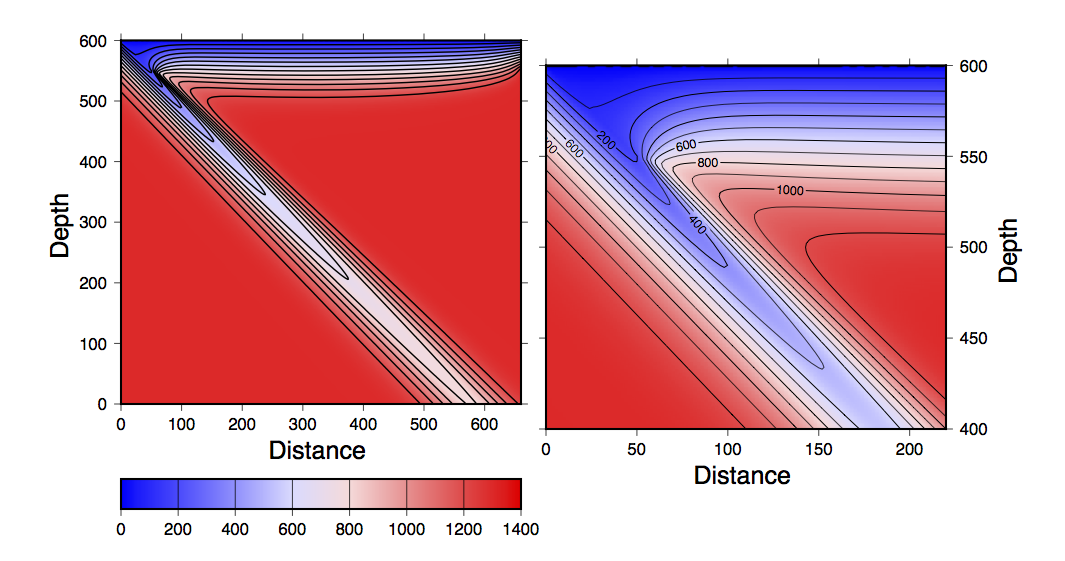
\includegraphics[width=6in]{images/vanKeken08_fig2.png} 
\caption{\label{fig:wedge} Thermal structure for the mantle wedge problem in Cookbook 2 example for 330 by 300 element grid with imposed Batchelor wedge inflow/outflow boundary conditions. Compare with \citet{vanKeken08} Figure 2.}
\end{centering}
\end{figure}

The subduction zone thermal benchmark requests output values specified at specific grid points and the user would be well advised to carefully read \citet{vanKeken08} for details.
From \citet{vanKeken08}, {\em to compare model results each group contributed the temperature field as discreted values $T_{ij}$ on an equidistant grid with 6~km spacing, which is a 111$\times$101 matrix stored row-wise starting in the top left corner. 
From this grid we have extracted the following measurements for direct comparison: (1) the temperature $T_{11,11}$ which is at coordinates (60, 60 km) and just down-stream from the corner point.}
Further, users are requested to provide the L2 norm of the slab-wedge interface temperature between 0 and 210 km depth defined by
\begin{equation}
    ||T_{slab}|| = \sqrt{\frac{\sum\limits_{i=1}^{36} {T_{ii}}^2}{36}},
\end{equation}
and the L2 norm of the temperature of the mantle wedge from 54 to 120~km depth,
\begin{equation}
    ||T_{wedge}|| = \sqrt{\frac{\sum\limits_{i=10}^{21}\sum\limits_{j=10}^{i} {T_{ij}}^2}{78}}.
\end{equation}
These quantities are reported in Table~\ref{tab:slab}.   
Comparing Table~~\ref{tab:slab} with the results in \citet{vanKeken08}, few observations can be made.
First, the results for $T_{11}$, $||T_{slab}||$, $||T_{wedge}||$ approach the result reported in \citet{vanKeken08} for ConMan and are within the range of values reported by the other codes ($379.87 < T_{11} < 396.3$, $502.26 < ||T_{slab}|| < 520.14$, and $ 825.89 < ||T_{wedge}|| < 866.52$ and for 1a.
For 1b and 1c, the wedge values are somewhat lower than most codes, yet are inline with the 1a result.
Previously the VT result (i.e., ConMan) was the lowest in the range of reported values, thus the results here are actually an improvement over the results reported in the benchmark.
The results reported in \citet{vanKeken08} used an irregular grid and the fault implementation was not as clean as the implementation here.
The next thing to note is that the low-resolution grid (66x60) results are more than 100 degress lower than the most refined grid for $T_{11}$ but the differences  are less pronounced for $||T_{slab}||$ and $||T_{wedge}||$.

\begin{table}
\centering
\begin{tabular} {| l r c c c r |} \hline 
\multicolumn{1}{| c }{Case} &
\multicolumn{1}{ c }{Grid} &
\multicolumn{1}{ c }{$T_{11}$} &
\multicolumn{1}{ c }{$||T_{slab}||$} &
\multicolumn{1}{ c }{$||T_{wedge}||$} &
\multicolumn{1}{ c |}{Time (sec)} \\ 
\hline 
 1a & 66x60 & 226.61 & 463.77 & 804.32 & 2.21 \\
 1a & 132x120 & 346.51 & 488.73 & 827.83 & 12.90 \\
 1a & 198x180 & 364.19 & 499.35 & 835.75 & 38.74 \\
 1a & 264x240 & 402.26 & 506.77 & 838.02 & 132.31 \\
 1a & 330x300 & 386.77 & 505.58 & 837.93 & 300.57 \\
\hline 
 1b & 66x60 & 193.49 & 381.30 & 686.77 & 2.50 \\
 1b & 132x120 & 262.84 & 438.60 & 770.27 & 10.22 \\
 1b & 198x180 & 288.47 & 463.42 & 797.87 & 44.29 \\
 1b & 264x240 & 415.82 & 511.40 & 840.80 & 135.43 \\
 1b & 330x300 & 387.50 & 500.64 & 833.42 & 321.01 \\
\hline 
 1c & 66x60 & 192.10 & 372.87 & 666.34 & 2.45 \\
 1c & 132x120 & 260.88 & 433.84 & 759.46 & 10.30 \\
 1c & 198x180 & 286.81 & 459.99 & 790.22 & 44.88 \\
 1c & 264x240 & 414.05 & 509.23 & 836.24 & 144.93 \\
 1c & 330x300 & 385.94 & 498.59 & 828.96 & 324.21 \\
\hline 
\end{tabular}
\caption{Slab thermal structure results from \citet{vanKeken08} benchmarks.\label{tab:slab}} 
\end{table}

It is instructive to look at the temperature along the top of the slab, plotted in Figure~\ref{fig:tos}.
It is notable that for the coarse grids (red, greeen, and blue lines), the imposed Batchelor velocity solution (solid lines, `a' cases), which is the true solution, and the calculations with the Batchelor boundary conditions (dotted lines,`b' cases) or natural boundary conditions (dashed lines, `c' cases) are far apart.
With increasing grid resolution, the difference between the imposed Batchelor velocity solution and the numerical velocity solution approach each other.

On the coarse grids, the under and over-shoot of the temperature (i.e., the saw-tooth pattern), is characteristic of an under-resolved solution.
SUPG elements can only do so much.
This behavior disappears as the grid is refined. 

\begin{figure}
\begin{centering}
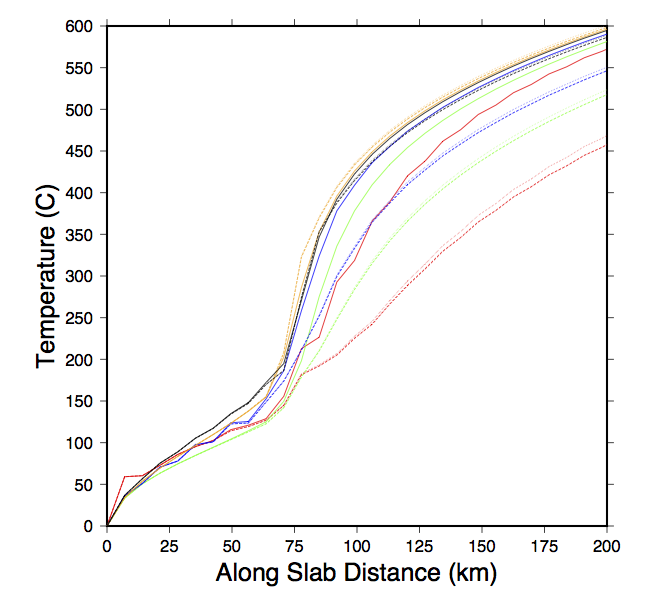
\includegraphics[width=5in]{images/tos.png} 
\caption{\label{fig:tos} Temperature along the top of the slab for the calculations in Table~\ref{tab:slab}.
Solid lines are for `a' cases, dotted lines are for `b' cases and dashed lines are for `c' cases.
The red lines are 66x60 element grids, the green lines are 132x120 element grids, the blue lines are 198x180 element grids, the orange lines are 264x240 element grids, and the black lines are for 330x300 element grids.}
\end{centering}
\end{figure}

To run the benchmark calculations use the scripts run\_66x60.sh, run\_132x120.sh, run\_198x180.sh, run\_264x240.sh, and run\_330x300.sh in the Cookbook2 subdirectory.
The scripts will run the three problems on the grid described in the script name and create plots (postscript) of the temperature and velocity fields using GMT.
(The plotting script is written for GMT5.)
If you do not have GMT on your system you can comment out the lines that contain the script plot\_temp\_GMT
Then the script Make\_table.sh will create a latex table of the results which should be identical to Table~\ref{tab:slab}.  
This script also uses GMT for the analysis.
The resulting file with the table will be vanKeken08.ps
You may need to edit Make\_table.sh to specify the location of latex and dvips if they are not already in your path.
Figure~\ref{fig:wedge} can be reproduced by running the script run\_330x300.sh and then Make\_vanKeken08\_fig2.sh.
The resulting file will be vanKeken08\_fig2.ps
To reproduce the plot of slab surface temperature, Figure~\ref{fig:tos}, run Make\_top\_of\_slab.sh.
The resulting postscript file will be tos.ps.

\section{Cookbook 3: Compressible Benchmark Cases from King {\em et al.} [2010]}

The benchmark problems are in unit-aspect ratio domain, with free-slip top, bottom, and sides walls.
The total temperature is fixed at the top $T(z=0) = 0$ and bottom $T(z=1) = 1$ and the side-walls have no flux boundary conditions.
We consider Bousinessq (BA), extended Bousinessq (EBA), truncated anelastic liquid (TALA) and anelastic liquid (ALA) approximations.
All thermodynamic properties are fixed constants.
The Rayleigh number, $Ra$, ranges from $10^4-10^6$ and we vary the Dissipation number, $Di$, from 0 to 2.
All of the cases in the test suite use 64 by 64 uniformly spaced elements.
All grids used in the benchmark are in the range of 60-128 elements (or nodes) per side.
We compared some solutions on more refined grids to check the convergence of the methods and error; however, the grids here are sufficient to resolve the problems in this study.
The participants were asked to report surface heat flux (Nusselt number) and rms velocity for all cases and in addition, the viscous dissipation and work done for the compressible cases.

The Nusselt number is a ratio of the average surface heat flow from the convective solution to the heat flow due to conduction and is calculated by
\begin{equation}
Nu = -\frac{1}{\lambda\Delta T} \int_{0}^{\lambda} \frac{\partial T^{\prime}(x,z=z_{top})}{\partial z}  dx,
\label{nu}
\end{equation}
where  $0$ and $\lambda$ are the left and right coordinates of the domain, respectively, $z_{top}$ is the top of the domain and, $\Delta T$ is the temperature contrast across the domain.
The rms velocity is given by 
\begin{equation}
V_{rms} = \frac{1}{\lambda (z_{top}-z_{bot})}\int_{z_{bot}}^{z_{top}} \int_{0}^{\lambda}  \left [(u^2 + w^2)  \right ]^{\frac{1}{2}} dx~~dz.
\label{vrms}
\end{equation}

In addition to the set of calculations described above, we added a series of temperature-dependent cases with a viscosity function 
\begin{equation}
\eta (T) = \eta_o \exp \left [ -\beta T \right ],
\label{tdep}
\end{equation}
where $\eta_o = 1$, $T$ is normalized by $ \Delta T = 3000.0 $ and $ \beta = \ln (1000) $, following problem 2a in \citet{blankenbach89}.
These calculations are in a unit-aspect ratio domain, with free-slip top, bottom, and sides walls.
Participants were asked to provide ALA results if possible and if not, TALA results.

In the directory Cookbook3 there is a shell script \emph{ RUN\_TEST\_SUITE } which runs a series of problems from the 2010 compressible benchmark paper.  
Each problem is in a subdirectory named in such a way that the problem is fairly obvious. 
Each of the constant viscosity problems runs in under 10 minutes and many run in under 2 minutes.  
The temperature-dependent problems run in under 2 hours.  
The entire test suite will run overnight on most systems (if you are impatient you can move the temperature-dependent problem directories to a name that starts with something other than `test') and the script will avoid running these.  
After the test suite is finished you can run Make\_table.bash (this assumes that you have latex and dvips installed).  
This will generate a table with your results and the expected values, and should look like the table below. 
You can view the resulting table on your system by typing <view> blankenbach.ps, where <view> is the software you use to view postscript files on your system.

\subsection{Boundary Conditions for Compressible Convection}

It is important to point out that boundary conditions for temperature require special care when compared with the more commonly used Bousinessq approximation.
In the description of this problem, the total temperature jump across the model is $\Delta T_r$ which is comprised of both a contribution from the reference state $\bar{T}$ and the potential temperature $T^{\prime}$.  The non-dimensional temperature at the surface, $T_o$ is given by $T_{surf}/ \Delta T_r$.
Because equation \ref{energyala} is written in terms of the potential temperature, $T^{\prime}$ the boundary conditions for equation \ref{energyala} are, $T^{\prime}(z=0) = 0$ and $T^{\prime}(z=1) = 1 - \exp(Di)$.  
This requires care when defining the Nusselt number, as discussed above.
The different codes used different formulations (e.g., CU formulation is based on total temperature, while the VT and UM formulations are based on potential temperature).
We do not internally modify the basal boundary condition in this formulation and the user must specify the boundary condition as $T_{bc} = 1-\exp(Di)$ in the \textbf{geom.} file. 

This table is a sample of the results from the test suite in Cookbook 3.  
For some of the cases, the results do not match the \citet{king10} results exactly.  
Additionally, \citet{king10} only report top Nusselt number and only report the temperature dependent results for the ALA case.
Here we report both the top and bottom Nusselt numbers, which provides a measure of the energy conservation.

There are several potential reasons for the disagreement: 1) there may have been rounding of some of the values reported in the supplemental table; 2) the results were computed from four separate versions of ConMan, one for each approximation, in the merged version the order of some of the operations differ substantially from the separate versions; 3) the small differences may reflect the cutoff at which the solution was judged to have converged; 4) for the $Ra=10^6$ case a refined grid was likely used.
The results here are consistent with those in Cookbook~1 and demonstrate that a substantially more refined grid is needed to achieve the rms velocity reported in \citet{king10} for this Rayleigh number.

The results here are consistent with the variations between codes reported in the benchmark paper and to the best of our knowledge are correct. 
There is a second script RUN\_PARALLEL.sh which checks for the number of CPUs on a multi-core system and runs up to that number of jobs simultaneously.
The steady-state diagnostics (v$_{rms}$, top and bottom Nusselt numbers, average temperature and surface velocity can be compared with the ConMan results in \citet{king10} by running the script Make\_table.sh.
The script assumes that latex and dvips are in your path and will produce a file named benchmark.ps.
An example of benchmark.ps is shown below.
The test results in Table~\ref{tab:compress} were computed on a MacBook Air with a 2.2 GHz Intel Core i7 processor running 10.11.6 (El Capitan) using gfortran (6.1.0) with compiler flags  -O3.

\noindent\rm
\begin{table}[h]
\centering
\begin{tabular} {| l c c c c c |} \hline 
\multicolumn{1}{| c }{Problem} &
\multicolumn{1}{ c }{V$_{rms}$} &
\multicolumn{1}{ c }{Nu Bot} &
\multicolumn{1}{ c }{Nu Top} &
\multicolumn{1}{ c }{ave T} &
\multicolumn{1}{ c |}{Vsurf} \\ 
\hline 
Blankenbach 1a explicit & 42.979 & 4.886 & 4.886 & 0.500 & 41.431 \\
Blankenbach 1a Picard & 42.979 & 4.886 & 4.886 & 0.500 & 41.431 \\
King et al. [2010] & 42.900 & - & 4.890 & 0.500 & 41.400 \\
\hline
Blankenbach 1b explicit & 194.768 & 10.540 & 10.540 & 0.500 & 198.282 \\
Blankenbach 1b picard & 194.768 & 10.540 & 10.540 & 0.500 & 198.282 \\
King et al. [2010] & 195.080 & - & 10.540 & 0.500 & 198.280 \\
\hline
Blankenbach 1c explicit & 846.728 & 22.017 & 22.017 & 0.500 & 884.520 \\
Blankenbach 1c picard & 846.729 & 22.017 & 22.017 & 0.500 & 884.520 \\
King et al. [2010] & 838.024 & - & 22.020 & 0.500 & 884.520 \\
\hline
Blankenbach 2a explicit & 493.066 & 10.076 & 10.071 & 0.741 & 98.760 \\
Blankenbach 2a Picard & 493.067 & 10.076 & 10.071 & 0.741 & 98.760 \\
King et al. [2010] & - & - & - & -  & - \\
\hline
EBA cv Di=0.25 explicit & 38.543 & 4.096 & 4.096 & 0.491 & 36.599 \\
EBA cv Di=0.25 Picard & 38.543 & 4.096 & 4.096 & 0.491 & 36.599 \\
King et al. [2010] & 38.476 & - & 4.097 & 0.491  & 36.598 \\
\hline
EBA cv Di=1.0 explicit  & 24.242 & 2.194 & 2.194 & 0.467 & 22.242 \\
EBA cv Di=1.0 Picard & 24.243 & 2.194 & 2.194 & 0.467 & 22.243 \\
King et al. [2010] & 24.232 & - & 2.194 & 0.467  & 22.243 \\
\hline
EBA td Di=0.25 explicit & 374.401 & 7.629 & 7.616 & 0.692 & 81.793 \\
EBA td Di=0.25 Picard & 374.401 & 7.629 & 7.616 & 0.692 & 81.795 \\
King et al. [2010] & - & - & - & -  & - \\
\hline
TALA cv Di=0.25 explicit & 40.163 & 4.426 & 4.424 & 0.513 & 39.301 \\
TALA cv Di=0.25 Picard & 40.163 & 4.426 & 4.425 & 0.513 & 39.301 \\
King et al. [2010] & 40.200 & - & 4.430 & 0.513 & 39.300 \\
\hline
TALA cv Di=1.0 explicit  & 26.072 & 2.567 & 2.505 & 0.509 & 26.432 \\
TALA cv Di=1.0 Picard & 26.072 & 2.567 & 2.505 & 0.509 & 26.432 \\
King et al. [2010] & 26.100 & - & 2.570 & 0.509  & 26.400 \\
\hline
TALA td Di=0.25 explicit & 383.222 & 7.813 & 7.740 & 0.706 & 82.928 \\
TALA td Di=0.25 Picard & 383.222 & 7.813 & 7.740 & 0.706 & 82.928 \\
King et al. [2010] & - & - & - & -  & - \\
\hline
ALA cv Di=0.25 explicit & 40.043 & 4.414 & 4.415 & 0.515 & 38.837 \\
ALA cv Di=0.25 Picard & 40.043 & 4.414 & 4.415 & 0.515 & 38.837 \\
King et al. [2010] & 40.095 & - & 4.414 & 0.515 & 38.837 \\
\hline
ALA cv Di=1.0 explicit & 24.983 & 2.472 & 2.473 & 0.510 & 24.401 \\
ALA cv Di=1.0 Picard & 24.983 & 2.472 & 2.473 & 0.510 & 24.402 \\
King et al. [2010] & 25.016 & - & 2.472 & 0.510  & 24.401 \\
\hline
ALA td Di=0.25 explicit & 380.059 & 7.735 & 7.683 & 0.707 & 81.095 \\
ALA td Di=0.25 Picard & 380.058 & 7.735 & 7.683 & 0.707 & 81.094 \\
King et al. [2010] & 381.690 & - & 7.710 & 0.707  & 81.090 \\
\hline 
\end{tabular}
\caption{Steady State, 2D, convection in a 1 by 1 box \citet{king10} benchmarks.\label{tab:compress}} 
\end{table}

\appendix
%dummy comment inserted by tex2lyx to ensure that this paragraph is not empty
%dummy comment inserted by tex2lyx to ensure that this paragraph is not empty
%dummy comment inserted by tex2lyx to ensure that this paragraph is not empty



\chapter{License }

\textbf{GNU GENERAL PUBLIC LICENSE Version 2, June 1991. Copyright
(C) 1989, 1991 Free Software Foundation, Inc. 59 Temple Place, Suite
330, Boston, MA 02111-1307 USA} \\
 Everyone is permitted to copy and distribute verbatim copies of this
license document, but changing it is not allowed.


\section*{Preamble}

The licenses for most software are designed to take away your freedom
to share and change it. By contrast, the GNU General Public License
is intended to guarantee your freedom to share and change free software
-- to make sure the software is free for all its users. This General
Public License applies to most of the Free Software Foundation's software
and to any other program whose authors commit to using it. (Some other
Free Software Foundation software is covered by the GNU Library General
Public License instead.) You can apply it to your programs, too.

When we speak of free software, we are referring to freedom, not price.
Our General Public Licenses are designed to make sure that you have
the freedom to distribute copies of free software (and charge for
this service if you wish), that you receive source code or can get
it if you want it, that you can change the software or use pieces
of it in new free programs; and that you know you can do these things.

To protect your rights, we need to make restrictions that forbid anyone
to deny you these rights or to ask you to surrender the rights. These
restrictions translate to certain responsibilities for you if you
distribute copies of the software, or if you modify it.

For example, if you distribute copies of such a program, whether gratis
or for a fee, you must give the recipients all the rights that you
have. You must make sure that they, too, receive or can get the source
code. And you must show them these terms so they know their rights.

We protect your rights with two steps:

\begin{enumerate}
\item Copyright the software, and 
\item Offer you this license which gives you legal permission to copy, distribute
and/or modify the software. 
\end{enumerate}
Also, for each author's protection and ours, we want to make certain
that everyone understands that there is no warranty for this free
software. If the software is modified by someone else and passed on,
we want its recipients to know that what they have is not the original,
so that any problems introduced by others will not reflect on the
original authors' reputations.

Finally, any free program is threatened constantly by software patents.
We wish to avoid the danger that redistributors of a free program
will individually obtain patent licenses, in effect making the program
proprietary. To prevent this, we have made it clear that any patent
must be licensed for everyone's free use or not licensed at all.

The precise terms and conditions for copying, distribution and modification
follow.


\section*{GNU GENERAL PUBLIC LICENSE TERMS AND CONDITIONS FOR COPYING, DISTRIBUTION
AND MODIFICATION }

\begin{itemize}
\item [0.] This License applies to any program or other work which contains
a notice placed by the copyright holder saying it may be distributed
under the terms of this General Public License. The \char`\"{}Program\char`\"{}
below refers to any such program or work, and a \char`\"{}work based
on the Program\char`\"{} means either the Program or any derivative
work under copyright law: that is to say, a work containing the Program
or a portion of it, either verbatim or with modifications and/or translated
into another language. (Hereinafter, translation is included without
limitation in the term \char`\"{}modification.\char`\"{}) Each licensee
is addressed as \char`\"{}you.\char`\"{}\\
 \\
 Activities other than copying, distribution and modification are
not covered by this License; they are outside its scope. The act of
running the Program is not restricted, and the output from the Program
is covered only if its contents constitute a work based on the Program
(independent of having been made by running the Program). Whether
that is true depends on what the Program does. 
\end{itemize}
\begin{enumerate}
\item You may copy and distribute verbatim copies of the Program's source
code as you receive it, in any medium, provided that you conspicuously
and appropriately publish on each copy an appropriate copyright notice
and disclaimer of warranty; keep intact all the notices that refer
to this License and to the absence of any warranty; and give any other
recipients of the Program a copy of this License along with the Program.


You may charge a fee for the physical act of transferring a copy,
and you may at your option offer warranty protection in exchange for
a fee.

\item You may modify your copy or copies of the Program or any portion of
it, thus forming a work based on the Program, and copy and distribute
such modifications or work under the terms of Section 1 above, provided
that you also meet all of these conditions:

\begin{enumerate}
\item You must cause the modified files to carry prominent notices stating
that you changed the files and the date of any change. 
\item You must cause any work that you distribute or publish, that in whole
or in part contains or is derived from the Program or any part thereof,
to be licensed as a whole at no charge to all third parties under
the terms of this License. 
\item If the modified program normally reads commands interactively when
run, you must cause it, when started running for such interactive
use in the most ordinary way, to print or display an announcement
including an appropriate copyright notice and a notice that there
is no warranty (or else, saying that you provide a warranty) and that
users may redistribute the program under these conditions, and telling
the user how to view a copy of this License. (Exception: if the Program
itself is interactive but does not normally print such an announcement,
your work based on the Program is not required to print an announcement.) 
\end{enumerate}
These requirements apply to the modified work as a whole. If identifiable
sections of that work are not derived from the Program, and can be
reasonably considered independent and separate works in themselves,
then this License, and its terms, do not apply to those sections when
you distribute them as separate works. But when you distribute the
same sections as part of a whole which is a work based on the Program,
the distribution of the whole must be on the terms of this License,
whose permissions for other licensees extend to the entire whole,
and thus to each and every part regardless of who wrote it.

Thus, it is not the intent of this section to claim rights or contest
your rights to work written entirely by you; rather, the intent is
to exercise the right to control the distribution of derivative or
collective works based on the Program.

In addition, mere aggregation of another work not based on the Program
with the Program (or with a work based on the Program) on a volume
of a storage or distribution medium does not bring the other work
under the scope of this License.

\item You may copy and distribute the Program (or a work based on it, under
Section 2) in object code or executable form under the terms of Sections
1 and 2 above provided that you also do one of the following:

\begin{enumerate}
\item Accompany it with the complete corresponding machine-readable source
code, which must be distributed under the terms of Sections 1 and
2 above on a medium customarily used for software interchange; or, 
\item Accompany it with a written offer, valid for at least three years,
to give any third party, for a charge no more than your cost of physically
performing source distribution, a complete machine-readable copy of
the corresponding source code, to be distributed under the terms of
Sections 1 and 2 above on a medium customarily used for software interchange;
or, 
\item Accompany it with the information you received as to the offer to
distribute corresponding source code. (This alternative is allowed
only for noncommercial distribution and only if you received the program
in object code or executable form with such an offer, in accord with
Subsection b above.) 
\end{enumerate}
The source code for a work means the preferred form of the work for
making modifications to it. For an executable work, complete source
code means all the source code for all modules it contains, plus any
associated interface definition files, plus the scripts used to control
compilation and installation of the executable. However, as a special
exception, the source code distributed need not include anything that
is normally distributed (in either source or binary form) with the
major components (compiler, kernel, and so on) of the operating system
on which the executable runs, unless that component itself accompanies
the executable.

If distribution of executable or object code is made by offering access
to copy from a designated place, then offering equivalent access to
copy the source code from the same place counts as distribution of
the source code, even though third parties are not compelled to copy
the source along with the object code.

\item You may not copy, modify, sublicense, or distribute the Program except
as expressly provided under this License. Any attempt otherwise to
copy, modify, sublicense or distribute the Program is void, and will
automatically terminate your rights under this License. However, parties
who have received copies, or rights, from you under this License will
not have their licenses terminated so long as such parties remain
in full compliance. 
\item You are not required to accept this License, since you have not signed
it. However, nothing else grants you permission to modify or distribute
the Program or its derivative works. These actions are prohibited
by law if you do not accept this License. Therefore, by modifying
or distributing the Program (or any work based on the Program), you
indicate your acceptance of this License to do so, and all its terms
and conditions for copying, distributing or modifying the Program
or works based on it. 
\item Each time you redistribute the Program (or any work based on the Program),
the recipient automatically receives a license from the original licensor
to copy, distribute or modify the Program subject to these terms and
conditions. You may not impose any further restrictions on the recipients'
exercise of the rights granted herein. You are not responsible for
enforcing compliance by third parties to this License. 
\item If, as a consequence of a court judgment or allegation of patent infringement
or for any other reason (not limited to patent issues), conditions
are imposed on you (whether by court order, agreement or otherwise)
that contradict the conditions of this License, they do not excuse
you from the conditions of this License. If you cannot distribute
so as to satisfy simultaneously your obligations under this License
and any other pertinent obligations, then as a consequence you may
not distribute the Program at all. For example, if a patent license
would not permit royalty-free redistribution of the Program by all
those who receive copies directly or indirectly through you, then
the only way you could satisfy both it and this License would be to
refrain entirely from distribution of the Program.


If any portion of this section is held invalid or unenforceable under
any particular circumstance, the balance of the section is intended
to apply and the section as a whole is intended to apply in other
circumstances.

It is not the purpose of this section to induce you to infringe any
patents or other property right claims or to contest validity of any
such claims; this section has the sole purpose of protecting the integrity
of the free software distribution system, which is implemented by
public license practices. Many people have made generous contributions
to the wide range of software distributed through that system in reliance
on consistent application of that system; it is up to the author/donor
to decide if he or she is willing to distribute software through any
other system and a licensee cannot impose that choice.

This section is intended to make thoroughly clear what is believed
to be a consequence of the rest of this License.

\item If the distribution and/or use of the Program is restricted in certain
countries either by patents or by copyrighted interfaces, the original
copyright holder who places the Program under this License may add
an explicit geographical distribution limitation excluding those countries,
so that distribution is permitted only in or among countries not thus
excluded. In such case, this License incorporates the limitation as
if written in the body of this License. 
\item The Free Software Foundation may publish revised and/or new versions
of the General Public License from time to time. Such new versions
will be similar in spirit to the present version, but may differ in
detail to address new problems or concerns.


Each version is given a distinguishing version number. If the Program
specifies a version number of this License which applies to it and
\char`\"{}any later version,\char`\"{} you have the option of following
the terms and conditions either of that version or of any later version
published by the Free Software Foundation. If the Program does not
specify a version number of this License, you may choose any version
ever published by the Free Software Foundation.

\item If you wish to incorporate parts of the Program into other free programs
whose distribution conditions are different, write to the author to
ask for permission. For software which is copyrighted by the Free
Software Foundation, write to the Free Software Foundation; we sometimes
make exceptions for this. Our decision will be guided by the two goals
of preserving the free status of all derivatives of our free software
and of promoting the sharing and reuse of software generally. 
\end{enumerate}

\subsection*{NO WARRANTY }

\begin{itemize}
\item [11.]BECAUSE THE PROGRAM IS LICENSED FREE OF CHARGE, THERE IS NO
WARRANTY FOR THE PROGRAM, TO THE EXTENT PERMITTED BY APPLICABLE LAW.
EXCEPT WHEN OTHERWISE STATED IN WRITING THE COPYRIGHT HOLDERS AND/OR
OTHER PARTIES PROVIDE THE PROGRAM \char`\"{}AS IS\char`\"{} WITHOUT
WARRANTY OF ANY KIND, EITHER EXPRESSED OR IMPLIED, INCLUDING, BUT
NOT LIMITED TO, THE IMPLIED WARRANTIES OF MERCHANTABILITY AND FITNESS
FOR A PARTICULAR PURPOSE. THE ENTIRE RISK AS TO THE QUALITY AND PERFORMANCE
OF THE PROGRAM IS WITH YOU. SHOULD THE PROGRAM PROVE DEFECTIVE, YOU
ASSUME THE COST OF ALL NECESSARY SERVICING, REPAIR OR CORRECTION. 
\item [12.]IN NO EVENT UNLESS REQUIRED BY APPLICABLE LAW OR AGREED TO
IN WRITING WILL ANY COPYRIGHT HOLDER, OR ANY OTHER PARTY WHO MAY MODIFY
AND/OR REDISTRIBUTE THE PROGRAM AS PERMITTED ABOVE, BE LIABLE TO YOU
FOR DAMAGES, INCLUDING ANY GENERAL, SPECIAL, INCIDENTAL OR CONSEQUENTIAL
DAMAGES ARISING OUT OF THE USE OR INABILITY TO USE THE PROGRAM (INCLUDING
BUT NOT LIMITED TO LOSS OF DATA OR DATA BEING RENDERED INACCURATE
OR LOSSES SUSTAINED BY YOU OR THIRD PARTIES OR A FAILURE OF THE PROGRAM
TO OPERATE WITH ANY OTHER PROGRAMS), EVEN IF SUCH HOLDER OR OTHER
PARTY HAS BEEN ADVISED OF THE POSSIBILITY OF SUCH DAMAGES. 
\end{itemize}

\section*{END OF TERMS AND CONDITIONS }


\subsection*{How to Apply These Terms to Your New Programs}

If you develop a new program, and you want it to be of the greatest
possible use to the public, the best way to achieve this is to make
it free software which everyone can redistribute and change under
these terms.

To do so, attach the following notices to the program. It is safest
to attach them to the start of each source file to most effectively
convey the exclusion of warranty; and each file should have at least
the \char`\"{}copyright\char`\"{} line and a pointer to where the
full notice is found. For example:

\begin{quote}
One line to give the program's name and a brief idea of what it does.
Copyright {\footnotesize © (}year) (name of author)

This program is free software; you can redistribute it and/or modify
it under the terms of the GNU General Public License as published
by the Free Software Foundation; either version 2 of the License,
or (at your option) any later version.

This program is distributed in the hope that it will be useful, but
WITHOUT ANY WARRANTY; without even the implied warranty of MERCHANTABILITY
or FITNESS FOR A PARTICULAR PURPOSE. See the GNU General Public License
for more details.

You should have received a copy of the GNU General Public License
along with this program; if not, write to the Free Software Foundation,
Inc., 59 Temple Place, Suite 330, Boston, MA 02111-1307 USA 
\end{quote}
Also add information on how to contact you by electronic and paper
mail.

If the program is interactive, make it output a short notice like
this when it starts in an interactive mode:

\begin{quote}
Gnomovision version 69, Copyright © year name of author Gnomovision
comes with ABSOLUTELY NO WARRANTY; for details type `show w'. This
is free software, and you are welcome to redistribute it under certain
conditions; type `show c' for details. 
\end{quote}
The hypothetical commands `show w' and `show c' should show the appropriate
parts of the General Public License. Of course, the commands you use
may be called something other than `show w' and `show c'; they could
even be mouse-clicks or menu items -- whatever suits your program.

You should also get your employer (if you work as a programmer) or
your school, if any, to sign a \char`\"{}copyright disclaimer\char`\"{}
for the program, if necessary. Here is a sample; alter the names:

\begin{quote}
Yoyodyne, Inc., hereby disclaims all copyright interest in the program
`Gnomovision' (which makes passes at compilers) written by James Hacker.

(signature of Ty Coon)\\
 1 April 1989 \\
 Ty Coon, President of Vice 
\end{quote}
This General Public License does not permit incorporating your program
into proprietary programs. If your program is a subroutine library,
you may consider it more useful to permit linking proprietary applications
with the library. If this is what you want to do, use the GNU Library
General Public License instead of this License.

\bibliography{ConMan.bib}

\end{document}
